% TODO: Figure out how to call those "programming experiences" (also is this a good name?)
%   the text uses "concrete, collaborative, interactive" - but this is a silly list
%   really, they are "cool" but how to say that.
%
% TODO: Also, what exactly goes into the list?
%
%
\documentclass[sigconf]{acmart}
%\documentclass[sigconf,review,anonymous]{acmart}

\usepackage{hhline,xcolor,colortbl}
\usepackage{fontawesome}
\usepackage{enumitem}
\usepackage{fancyvrb}
\usepackage{tikz}
%\usepackage[breakable,theorems,skins]{tcolorbox}
%\usepackage{lettrine}
\usepackage{float}
\usepackage{hyperref}

\setlength{\marginparwidth}{1.4cm}

%\newcommand{\diff}[1]{{\textcolor{magenta}{#1}}}
%\newcommand{\note}[1]{\marginpar{\raggedright\scriptsize\textcolor{magenta}{#1}}}

\newcommand{\diff}[1]{{#1}}
\newcommand{\note}[1]{}

\newcommand{\ident}[1]{{\sffamily #1}}
\newcommand{\srcid}[1]{\textnormal{\sffamily #1}}
\newcommand{\srckvd}[1]{\textnormal{\sffamily\bfseries #1}}

\newcommand*\circled[1]{\textnormal{\footnotesize\sffamily\bfseries\protect\tikz[baseline=(char.base)]{
  \node[shape=circle,fill=black,text=white,draw,inner sep=1pt] (char) {#1};}}}

% \DeclareRobustCommand{\keyideabox}[3]{\begin{tcolorbox}[breakable,
%   boxsep=5pt,left=0pt,right=0pt,top=0pt,bottom=0pt,width=\dimexpr\columnwidth\relax,
%   colback=gray!20,colframe=gray!20,
%   enlarge bottom by=0pt,enlarge top by=0pt,
%   arc=0pt,outer arc=0pt]
% \lettrine[lraise=0.3]{\LARGE #1}{~}
% \small \textbf{#2.} #3
% \end{tcolorbox}
% }
\DeclareRobustCommand{\keyideabox}[3]
{\vspace{\dimexpr\baselineskip\relax} \noindent\colorbox{gray!20}{
\parbox{\dimexpr\columnwidth-\marginparsep+1pt\relax}
{\small {#1} \textbf{#2.} #3}
}}

\setlist{leftmargin=1.5em}
\setlength\itemsep{0.5em}

\copyrightyear{2025}
\acmYear{2025}
\setcopyright{cc}
\setcctype{by}
\acmConference[UIST '25]{The 38th Annual ACM Symposium on User Interface Software and Technology}{September 28-October 1, 2025}{Busan, Republic of Korea}
\acmBooktitle{The 38th Annual ACM Symposium on User Interface Software and Technology (UIST '25), September 28-October 1, 2025, Busan, Republic of Korea}\acmDOI{10.1145/3746059.3747646}
\acmISBN{979-8-4007-2037-6/2025/09}

\begin{document}
\title[Denicek: Computational Substrate for Document-Oriented End-User
  Programming]{{\scshape Denicek}: Computational Substrate for\\ Document-Oriented End-User Programming}

\author{Tomas Petricek}
\email{tomas@tomasp.net}
\orcid{0000-0002-7242-2208}
\affiliation{%
  \institution{Faculty of Mathematics and Physics, Charles University}
  \city{Prague}
  \country{Czech Republic}
}

\author{Jonathan Edwards}
\email{jonathanmedwards@gmail.com}
\orcid{0000-0003-1958-7967}
\affiliation{%
  \institution{Independent}
  \city{Boston}
  \country{USA}
}

\begin{abstract}
\note{Added overview figure with examples showing relationships between Denicek \& co.}
User-centric programming research gave rise to a variety of compelling programming experiences,
including collaborative source code editing, programming by demonstration, incremental
recomputation, schema change control, end-user debugging and concrete programming.
Those experiences advance the state of the art of end-user programming, but they are hard to
implement on the basis of established programming languages and system.

We contribute Denicek, a computational substrate that simplifies the implementation of the
above programming experiences. Denicek represents a program as a series of edits
that construct and transform a document consisting of data and formulas. Denicek provides three
operations on edit histories: edit application, merging of histories and conflict resolution.
Many programming experiences can be easily implemented by composing these three operations.

We present the architecture of Denicek, discuss key design considerations and elaborate
the implementation of a variety of programming experiences. To evaluate the proposed
substrate, we use Denicek to develop an innovative interactive data science notebook system.
The case study shows that the Denicek computational substrate provides a suitable basis for
the design of rich, interactive end-user programming systems.
\end{abstract}

\begin{CCSXML}
 <ccs2012>
    <concept>
        <concept_id>10011007.10011006.10011066</concept_id>
        <concept_desc>Software and its engineering~Development frameworks and environments</concept_desc>
        <concept_significance>500</concept_significance>
        </concept>
    <concept>
        <concept_id>10003120.10003121.10003129.10011756</concept_id>
        <concept_desc>Human-centered computing~User interface programming</concept_desc>
        <concept_significance>300</concept_significance>
        </concept>
    <concept>
        <concept_id>10003120.10003121.10003124.10010868</concept_id>
        <concept_desc>Human-centered computing~Web-based interaction</concept_desc>
        <concept_significance>300</concept_significance>
        </concept>
  </ccs2012>
\end{CCSXML}

\ccsdesc[500]{Software and its engineering~Development frameworks and environments}
\ccsdesc[300]{Human-centered computing~User interface programming}
\ccsdesc[300]{Human-centered computing~Web-based interaction}

\keywords{Programming Systems, End-User Programming}
%Computational Substrate,  Programming by Demonstration, Local-First Software}

\begin{teaserfigure}
  \vspace{0.25em}
  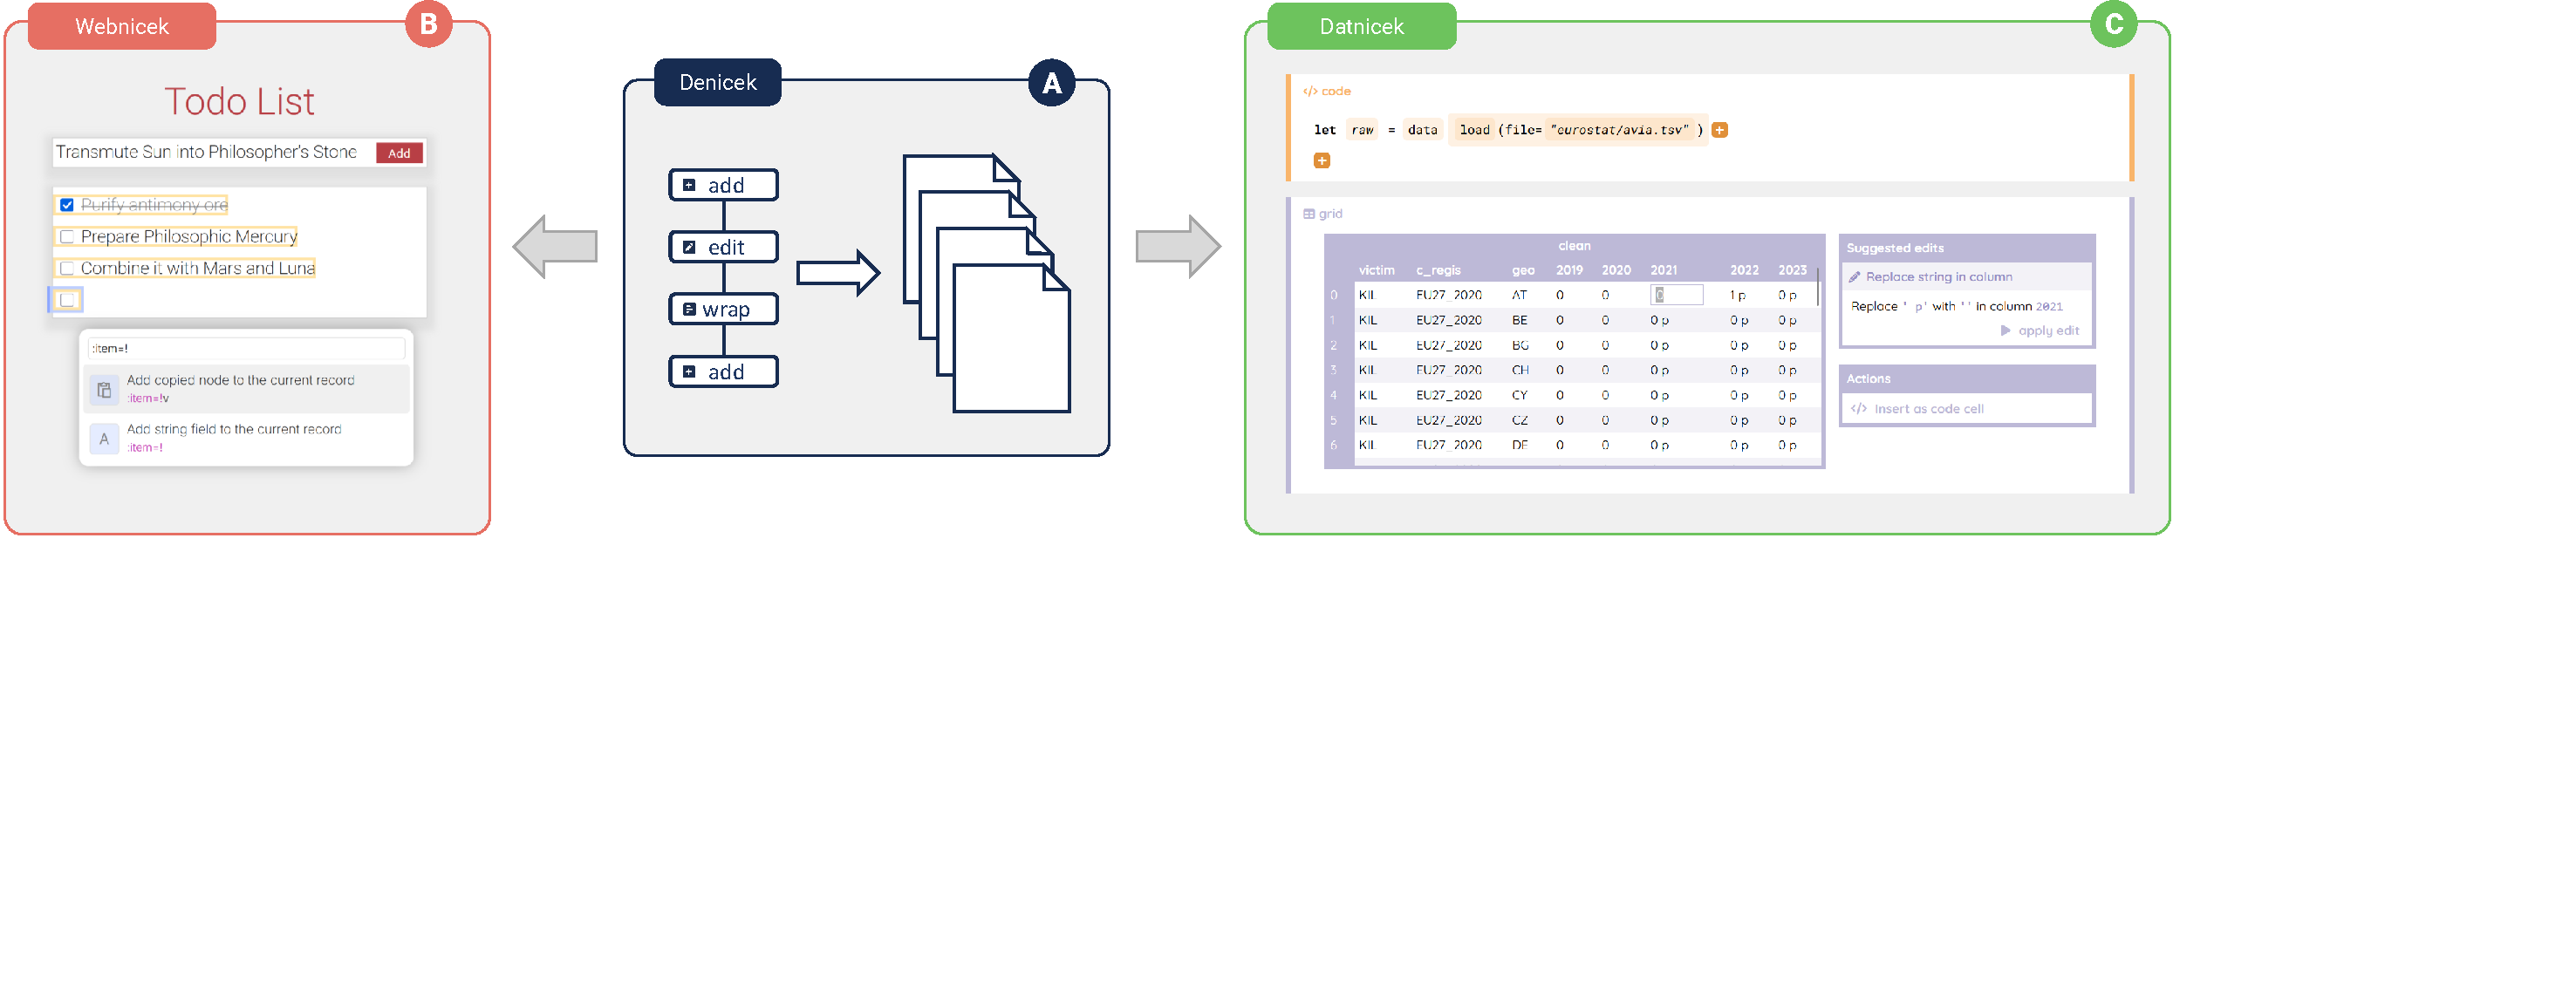
\includegraphics[width=1\textwidth,clip,trim=0cm 8.5cm 7.7cm 0cm]{fig/teaser.pdf}
  \vspace{-1.5em}
  \caption{\diff{Denicek is a computational substrate for document-oriented programming
    based on document edit histories~(A). We co-design Denicek with a web-based end-user
    programming environment Denicek (B). Here, Denicek is used to build a Todo list app via
    programming-by-demonstration, by copying a value from input to a new list item.
    We then evaluate the generality of Denicek by using it to build a data science notebook
    system Datnicek (C). Here, Datnicek is used to interactively clean the data table, by
    removing the `` p'' (provisional) marker from numerical columns.
  }}
  \Description{The Denicek diagram in the middle illustrates a document representation as an
   edit history. Two arrows point from the diagram to two screenshots. Webnicek on the left
   contains a Todo list app with a command toolbox showing add item operation. Datnicek on the
   right contains two cells, one with code to load data and another with an interactive editor
   for data cleaning.}
  \label{fig:teaser}
  \vspace{0.75em}
\end{teaserfigure}
\maketitle

% ==================================================================================================
\section{Introduction}

A computational substrate defines the structures with which programs are constructed, how
the program state is represented and how the state evolves during execution \cite{jakubovic-2022-ladder}.
The choice of a substrate affects what programming experiences can be readily supported.
For example, object-oriented programming has been historically linked to graphical user
interfaces~\cite{kay-1993-smalltalk}, while representing programs as lists enabled Lisp to become
a language laboratory~\cite{steele-1993-lisp}.

In principle, any programming experience can be developed on top of any computational
substrate. However, a suitable program representation can eliminate much of the complexity of implementing interesting
programming experiences. For example, the reflective capabilities of Smalltalk make it easy
to build rich debugging tools \cite{rauch-2019-babylonian} that are difficult to implement
for C/C++~\cite{kell-2018-unix,kell-2024-debugging}.

\subsubsection*{Programming Experiences}

\note{Revised to say Denicek is a substrate used to build programming systems.}
\diff{We describe Denicek, a computational substrate that makes it easy to build programming systems
supporting diverse compelling programming experiences \cite{myers-2006-eup}:}

\begin{itemize}
\item \emph{Collaborative Editing.} Users should be able to locally modify a shared document
  and merge their changes, preferably in a way that does not require a live connection to a central server~\cite{kleppmann-2019-local}.
\item \emph{Programming by Demonstration.} Allow users to construct simple programs by
  enacting the steps of the desired behavior using concrete examples and generalizing from the example~\cite{leiva-2021-rapido,cypher-1993-pbd}.
\item \emph{Incremental Recomputation.} When a part of a document changes, formulas whose result
  depends on the part are invalidated and, possibly automatically, recomputed \cite{teitelbaum-1981-cps,mcdirmid-2013-usable,horowitz-2023-engraft}.
\item \emph{Schema Change Control.} When the user evolves the structure of the document, affected
  data and formulas should automatically co-evolve to match the new structure~\cite{litt-2020-cambria,edwards-2025-schema}.
\item \emph{End-User Debugging.} The user should be able to ask provenance questions~\cite{cheney-2009-provenance} to understand
  why a computation resulted in a particular value and what inputs contributed to the result \cite{ko-2009-whyline}.
\item \emph{Concrete Programming.} It should be possible to reuse parts of program logic, or formulas,
  without introducing abstractions, that is, program against concrete values \cite{edwards-2006-copypaste,edwards-2022-copypaste}.
\end{itemize}

\subsubsection*{Two-Phase Methodology}
The technical focus of this paper fits within the interior mode of design science research \cite{adam-2021-dsr}.
To \emph{design} Denicek (Fig.~\ref{fig:teaser} (A)), we identify six \emph{formative examples} -- simple programming
tasks that manifest one or more of the desired programming experiences~(\S\ref{app:examples}).
Using those examples, we co-design the Denicek substrate and a simple web-based end-user programming
environment Webnicek~(Fig.~\ref{fig:teaser} (B)), which is built directly on top of the substrate. Although
Webnicek can be used to complete end-user programming tasks, it is optimized for developing the
underlying substrate rather than for usability.

To \emph{evaluate} the usability of Denicek for the development of end-user programming systems,
we use it to build Datnicek (Fig.~\ref{fig:teaser}~(C)), an innovative interactive data science notebook
that brings together a range of recent research work~\cite{kandel-2011-wrangler,drossos-2020-wrex,petricek-2022-thegamma,adams-2025-grove}.
\note{Clarify that Datnicek was designed after Denicek was completed.}
\diff{We reflect on the degree to which Denicek simplifies the implementation of a programming
system that is based on current research advances and was conceived after the design of Denicek
has been fully finalized~(\S\ref{sec:case-reflection}).} We also provide a heuristic evaluation
of Denicek characteristics including importance and generality (\S\ref{sec:eval}).

\subsubsection*{Computational Substrates}
Denicek brings together two central design ideas. First, it represents programs as
document trees consisting of nodes that can represent data, formulas, evaluated results, as well as
static content. Second, Denicek does not store the document tree itself, but instead, maintains
a sequence of edit operations through which the tree was constructed and transformed.

The substrate then provides three primitive operations for working with sequences of edits.
First, it can apply a series of edits to reconstruct the document. Second, it can merge two
diverging edit histories. Finally, it can detect conflicts when merging histories and, for
example, remove conflicting edits from one branch.

\subsubsection*{Key Takeaways}
\note{Add more general takeaway (below) and clarify specific technical takeaway (here).}
\diff{The key insights of this paper are twofold. A specific technical takeaway is that many
compelling programming experiences can be implemented on top a uniform document representation,
by using a suitable composition of three primitive operations that operate on sequences of
edit operations.}

Editing of data and formulas is done using a single set of primitive edit operations that
manipulate the document. A user-interface may provide a specialized editor, but still
trigger the primitive edits behind the scenes. Interacting with elements in the document,
such as a entering text in a textbox can also generate a document edit that can be merged or checked
for conflicts (\S\ref{sec:impl-interaction}).

As we will see, past edits that demonstrate an operation done with the
document can be recorded, allowing programming by demonstration (\S\ref{sec:impl-pbd}).  Replaying
such recorded edits is implemented using the merging operation, which means that recorded operations
continue working even if the document structure later evolves. Moreover, structural changes to the
document can be merged with concurrent data edits  (\S\ref{sec:impl-collab}). Evaluation of formulas
also generates document edits (\S\ref{sec:impl-eval}). If the evaluated edits conflict with manual
edits done later by the user, the evaluated edits are removed, yielding an incremental
recomputation behavior (\S\ref{sec:impl-incremental}).

\note{Add a more general takeaway suggested by Reviewer 3 (Thank you!)}
\diff{A more basic takeaway, illustrated by the development of Denicek, is that it is worth looking
for novel computational substrates that better support compelling programming experiences developed
in user-centric programming research.}

\subsubsection*{Contributions}
The structure and contributions of this paper are:

\begin{itemize}
\item We present the Denicek substrate (\S\ref{sec:system}) and provide a detailed description of its
  document representation, edit operations and the key three operations for working with edit histories.
\item We illustrate a range of end-user programming experiences supported in Webnicek, a simple
  web-based prototype programming system (\S\ref{sec:walk}), and discuss how the experiences are
  implemented on top of the Denicek substrate (\S\ref{sec:impl}).
\item We document important design decisions, alternatives and limitations (\S\ref{sec:discuss}).
  The analysis shows that the desired functionality requires a careful choice among interconnected
  design options.
\item To evaluate how Denicek simplifies the development of program\-ming systems, we
  build an innovative data science notebook Datnicek and assess its implementation
  complexity~(\S\ref{sec:case}). We also present heuristic evaluation of the system (\S\ref{sec:eval}).
\end{itemize}

\noindent
To enable others build on top of Denicek, we share our compact open-source
implementation at: \url{https://github.com/d3sprog/denicek}

% ==================================================================================================

\section{Background}
\label{sec:background}
\note{Clarify focus to make paper more self-contained}
\diff{The premise of Denicek is that suitable structures for constructing programs can make it easier
to support a range of compelling user experiences. A prime example is
Smalltalk whose object-oriented structures
enable malleable programming experience~\cite{girba-2017-moldable,tcher-2019-malleable}.}

Denicek aims to support a class of systems associated with end-user programming, liveness and
interactivity \cite{myers-2006-eup,horowitz-2023-qualities,rein-2019-live}, notational freedom and
self-sustainability~\cite{jakubovic-2023-techdims}. We see programming as interacting with a medium
or a substrate \cite{kay-1977-media,klokmose-2015-webstrates,rpg-2012-revolution} and
use the term end-user programming loosely to refer to a part of this spectrum, also including
spreadsheet systems and notebooks for data science.

\note{Highlight related systems (discussed later) for better framing}
\diff{We follow systems such as BootstrapLab~\cite{jakubovic-2022-ladder}, which aims to support
gradual progression from a user to a developer envisioned in Smalltalk~\cite{reenskaug-1981-byte}
in a primarily graphical environment and Subtext~\cite{edwards-2005-subtext},
which develops a user-friendly programming environment based on object copying.}

% --------------------------------------------------------------------------------------------------

\subsection{Programming Systems}
\label{sec:background-sys}

\subsubsection*{Programming Systems and Substrates}
A number of systems illustrate the qualities Denicek aims to support and have a related underlying
structure. Subtext, BootstrapLab and Infra~\cite{edwards-2005-subtext,jakubovic-2022-ladder,hall-2017-infra}
use structured document-based program representation and provide some of the desired programming
experiences on top of this representation. Many of those design ideas can be traced back to
Boxer~\cite{disessa-1986-boxer}, which introduced the \emph{naive realism} principle (what the user
sees is all there is) that we also follow in Webnicek.

To indicate that Denicek is intended as an underlying infrastructure on top of which programming
systems can be built, we use the term \emph{computational substrate}. The term also dates back to
Boxer~\cite{disessa-1995-epistemology} and is related to the notion of dynamic media of Kay and
Goldberg \cite{kay-1977-media}. Webstrates \cite{klokmose-2015-webstrates}
revisit the idea, providing a substrate based on synchronization of documents (without edit
histories) that has been used as the basis for multiple programming systems \cite{radle-2017-codestrates,borowski-2022-varv}.

\subsubsection*{Edit Histories and Merging}
Manipulating programs through semantically meaningful edits is a technique used by structure
editors \cite{teitelbaum-1981-cps,hempel-2018-deuce,beckman-2023-sandblocks}. The language of
edits has been captured formally as an \emph{edit calculus} \cite{omar-2017-hazelnut} and
edit histories have also been recognized as a suitable basis for live programming environments \cite{storm-2013-deltas}.

Merging of edits is most frequently done in version control systems. The
Pijul system \cite{meunier-2024-pijul} delays merging to a later point
by using a graph or a lattice \cite{schurmann-2022-merging}. In the context of
programming environments, Grove \cite{adams-2025-grove} uses a commutative patches with a similar graph
structure as the basis for a collaborative structure editor. \diff{Grove patches
(construct, delete, relocate) are sufficient for a structure editor, but lack some structures and
operations that our formative examples rely on (collections, copying). However, the core model
of Grove provides a possible alternative basis for Denicek.}
\note{Added why Grove cannot be used directly by Denicek, but is interesting direction.}

More generally, merging of edits can use the operational transform (OT) approach
\cite{davis-2002-otsgml}, where edit conflicts are reconciled, or conflict-free
representation (CRDTs) \cite{shapiro-2011-crdts,litt-2022-peritext}. The latter is commonly associated
with local-first software \cite{kleppmann-2019-local} that operates without a central server.
In both approaches, supporting complex edits on tree structures
remains a challenge \cite{jungnickel-2016-otjson,da-2024-jsoncrdt}. Mergeable replicated data
types (MRDTs) \cite{kaki-2019-mrdts} merge updates using a suitable relational
representation. Recent work on MySubstrates and Grove \cite{adams-2025-grove,klokmose-2024-mywebstrates}
has been based on CRDTs, whereas Edwards et al. \cite{edwards-2021-typed} prefer OT.

\note{Added report of our experience with what makes EUP systems hard to build.}
\subsubsection*{Building Programming Experiences}
\diff{
The challenge addressed by Denicek is that end-user programming experiences are hard to~build.
Our experience developing such systems \cite{petricek-2019-histogram,petricek-2022-thegamma,
jakubovic-2022-ladder,edwards-2005-subtext,edwards-2004-example} suggests two difficulties.
The first is the need to move between the concrete and the abstract \cite{jakubovic-2023-techdims}.
A sequence edits strikes a balance between those opposing representations.
The second is the need to combine multiple experiences, which requires
a major engineering effort when using a conventional program representation.}

% Wrangler~\cite{kandel-2011-wrangler}

% * Reviewers also ask about the concrete problem addressed (R2) and what makes end-user programming
% tools hard to build (R1). The latter question (aptly phrased by R1) deserves a deeper investigation.
% We believe the difficulty emerges when combining multiple programming experiences in a single system
% and from the need to move between the concrete and the abstract. This belief is based on our personal
% experience developing multiple systems (to be cited in the revision) and on a technical dimensions
% analysis (Sec. 8.2). A substrate based on edit history provides a middle ground between the
% abstract and the concrete and we show that it can be carefully designed to serve as the basis for a range of experiences.

% --------------------------------------------------------------------------------------------------

\begin{figure*}[t]
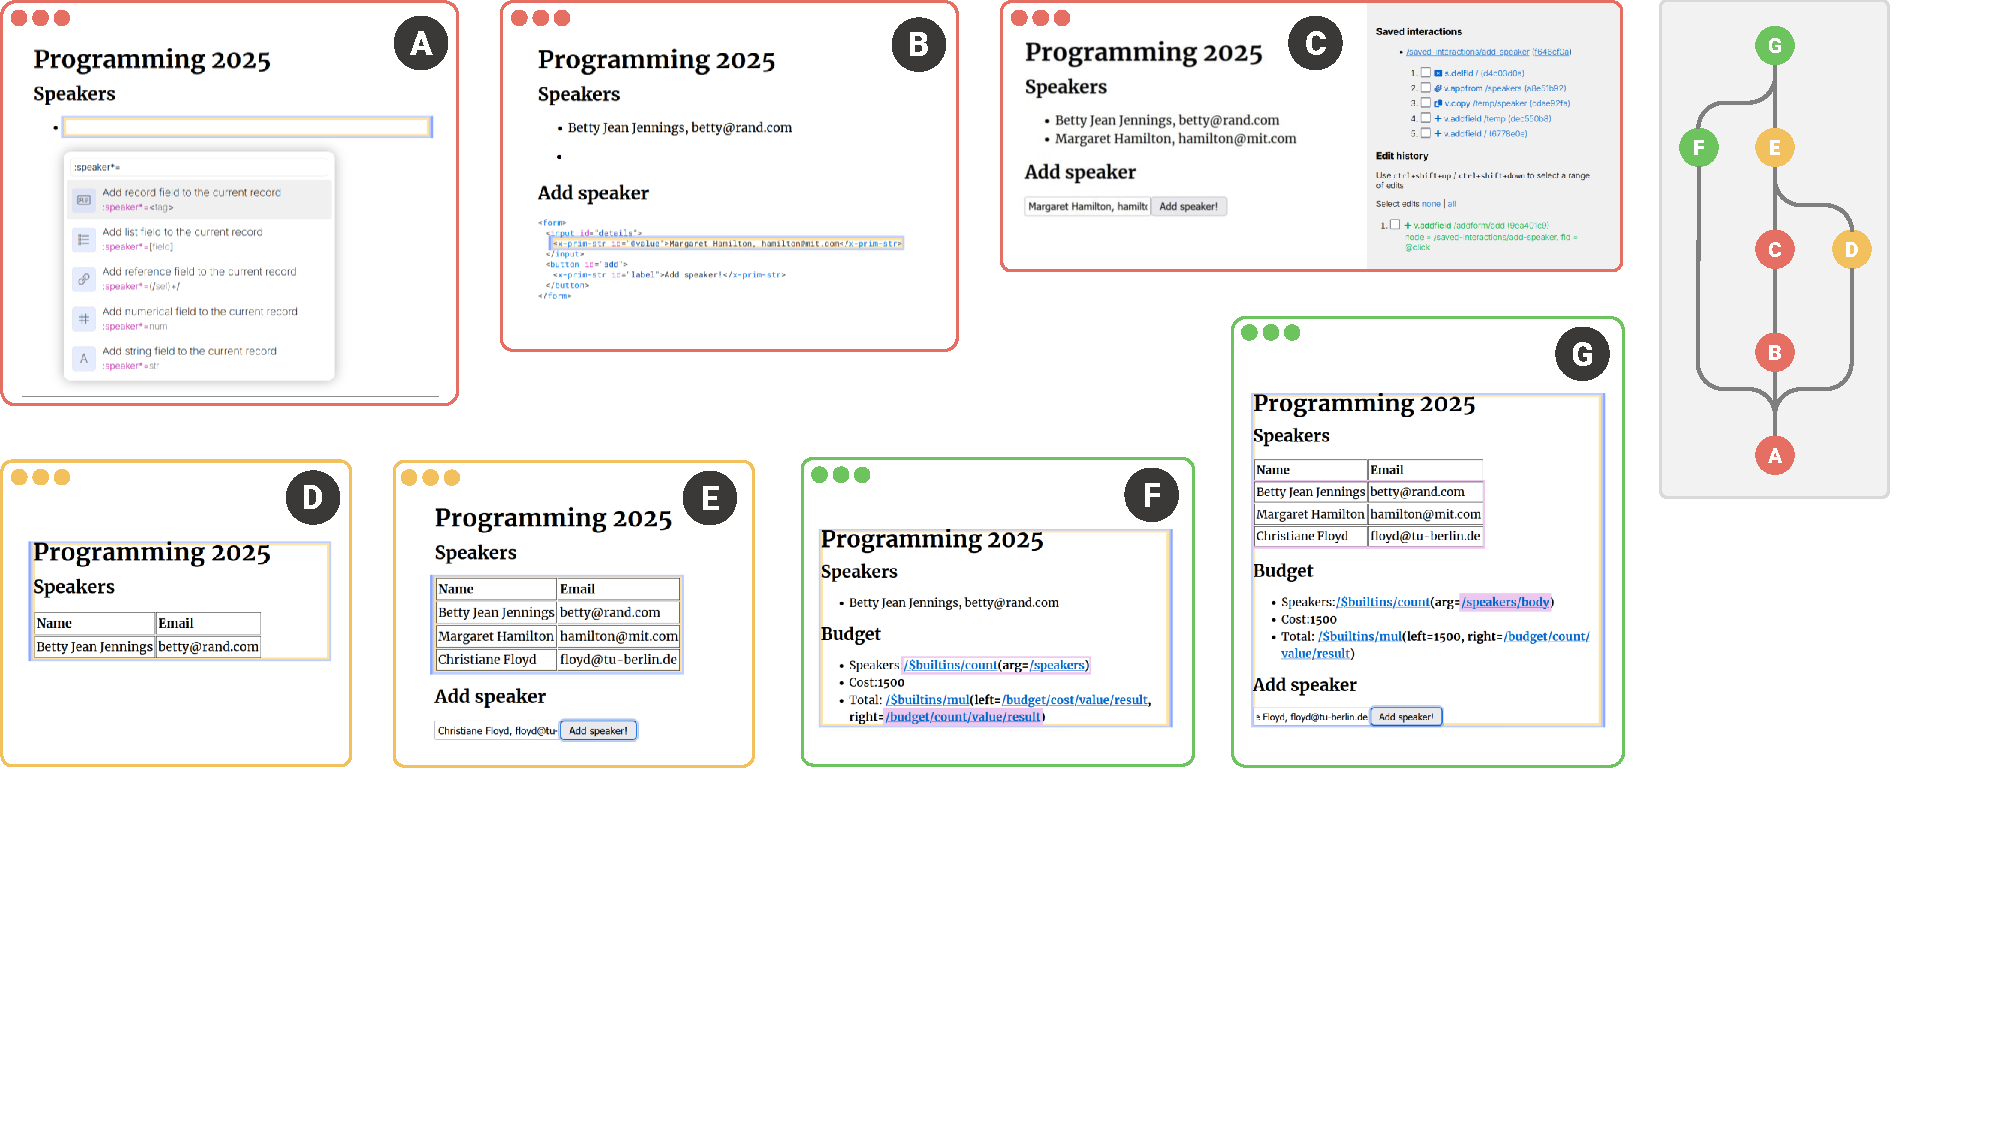
\includegraphics[width=0.95\textwidth,clip,trim=0cm 6cm 1.7cm 0cm]{fig/walkthrough.pdf}
% \vspace{-0.5em}
\caption{Organizing a conference using Denicek. The Walkthrough shows construction of a user
  interface for adding speakers (A, B, C); refactoring of the list and merging edits (D, E); and
  formulas with schema and code co-evolution (F, G).}
\label{fig:walkthrough}
\end{figure*}

% --------------------------------------------------------------------------------------------------

\subsection{Programming Experiences}
\label{sec:background-exp}

%We review a range of compelling programming experiences explored in recent research,
%focusing on those supported by Denicek.

\subsubsection*{Collaborative Editing}
Since the early collaborative programming environments such as Collabode \cite{goldman-2011-collaborative},
real-time collaboration has became widely used, if not always without challenges \cite{tan-2024-vslive}.
Merging concurrent edits is one such challenge. In addition to OT-based and CRDT-based
approaches \cite{klokmose-2024-mywebstrates}, conflicts arising during
collaboration have also been solved using fine-grained locking \cite{wang-2024-nbconflicts}.

\subsubsection*{Programming by Demonstration}
Earliest PbD systems used the paradigm for tasks ranging from graphics
and user interfaces to general-purpose programming \cite{smith-1975-pygmalion,cypher-1993-pbd}.
Wrangler \cite{kandel-2011-wrangler} showed the effectivity of PbD for data cleaning,
whereas more recent uses range from augmented reality prototyping \cite{leiva-2021-rapido}
and web automation \cite{chen-2023-miwa} to end-user software customization
\cite{litt-2020-customization,litt-2020-wildcard}. Expressing conditions in PbD remains an
active research topic~\cite{pu-2022-semanticon,radensky-2018-conditionals}. A more general class of demonstrational
interfaces \cite{myers-2000-intelligence} also includes programming by example, used
for example for data transformation in spreadsheets \cite{gulwani-2012-spreadsheets}.
Demonstrational interfaces can be used to directly perform actions, but also to generate code
as in Wrex \cite{drossos-2020-wrex}.

\subsubsection*{Incremental Recomputation}
Interactive programming systems with live previews \cite{petricek-2020-live,mcdirmid-2013-usable}
have been attempting to update the previews without full recomputation at least since the pioneering
work on the Cornell Program Synthesizer \cite{teitelbaum-1981-cps}. Outside live programming,
more work has been focused on updating computation when data change, although such data can also
be source code passed to an adaptive interpreter \cite{acar-2006-adaptive}.
Incremental recomputation is also a concern in notebook systems where cells can be run out of
order \cite{singer-2020-jollity}. The ordering problem can be addressed using a dependency graph
\cite{petricek-2018-wrattler,koop-2017-dataflow}, allowing for incremental recomputation
on code change.

\subsubsection*{Schema Change Control}
Schema change control is concerned with adapting data and code to reflect changes in schema.
The problem is well-studied in the context of databases \cite{brahmia-2024-evolution},
although only few systems also automatically adapt database queries \cite{wang-2019-schema}.
The problem is starting to be recognized in programming systems research
\cite{litt-2020-cambria,edwards-2025-schema} as well as live programming \cite{barenz-2020-live}
where state needs to be preserved during program editing.

\subsubsection*{End-User Debugging}
Non-programmers also need to be able understand and debug their programs \cite{kissinger-2006-debugging}.
Systems such as Whyline and Probe Log \cite{ko-2004-whyline,ko-2009-whyline,krebs-2023-probelog}
record information about program execution to let users analyse why they see a particular result,
whereas displaying intermediate steps can aid understanding of data science pipelines \cite{shrestha-2021-unravel}.
More generally, such functionality can leverage provenance tracking \cite{cheney-2009-provenance}
and program slicing \cite{ricciotti-2017-imperative,perera-2012-functional}. The same infrastructure
can also be used to build linked visualizations \cite{perera-2022-linked}.

\subsubsection*{Concrete Programming}
Programming can be simplified by working with concrete values instead of abstractions, an idea
pioneered by the prototype-based programming language Self \cite{ungar-1987-self}. In Self,
prototypes are used at the object level. At the expression level, similar functionality can be provided
by managed copy \& paste. Subtext \cite{edwards-2006-copypaste,edwards-2022-copypaste} treats this
mechanism as central, whereas other systems view tracking of copy \& paste as an extra
editor feature \cite{jablonski-2007-cren,toomim-2004-linked}. Copy \& paste has also been
tracked in spreadsheets \cite{hermans-2015-copypaste}. Gridlets \cite{joharizadeh-2020-gridlets}
offer a spreadsheet abstraction based on reusing concrete computation, similar to the one proposed
for The Gamma~\cite{petricek-2020-live}.

\subsubsection*{Other Programming Experiences}
Several experiences not directly addressed in this paper are worth further investigation.
Projectional editors such as Lorgnette \cite{gobert-2023-lorgnette},
live literals \cite{omar-2021-livelits}, projection boxes \cite{lerner-2020-boxes} and data detectors
\cite{nardi-1998-agents} allow visualization or editing of aspects of programs through a user interface.
The problem of making live and rich editors compositional is addressed by
Engraft \cite{horowitz-2023-engraft}. Programming environments may be also improved by integrating
live examples \cite{rauch-2019-babylonian} and a variety of AI assistance
tools \cite{petricek-2023-aias,blinn-2024-llms,mcnutt-2023-nbai}.


% ==================================================================================================

\section{Walkthrough}
\label{sec:walk}

We use the web-based prototype Webnicek to illustrate programming experiences enabled by Denicek.
Webnicek is based on a structure editor that supports navigation in the document and issuing of
edit commands. \diff{We follow a formative example (\S\ref{app:examples}) where Evelyn, Juliana and Alfred
collaboratively plan a conference.}
\note{Turn this into a concrete user story consistent with the video. Also add more details about
the edit operations and UI interactions.}

\subsubsection*{\circled{A} Adding a Speaker}
Evelyn starts with an empty document, which is represented as a record. She adds a field for
each heading and a field named {\small\Verb_speakers_} containing a list {\small\Verb_<ul>_}. \diff{She
uses the command toolbox to issue edit commands that add the first speaker.}

\subsubsection*{\circled{B} Creating a User Interface} To simplify adding of
further speakers, Evelyn creates a textbox and a button \diff{using the command toolbox}. She enters
the details of another speaker \diff{into the textbox}, adds a new {\small\Verb_<li>_} element
and copies the speaker details from the textbox into the new element in the source view,
\diff{using a copy command}.

\subsubsection*{\circled{C} Abstracting the Interaction} After adding the speaker,
Evelyn opens the history view, selects edits that added the speaker and saves them as the
{\small\Verb_add-speaker_} interaction. She attaches this interaction as an event handler for the
{\small\Verb_click_} event of the button.

\keyideabox{\faLightbulbO}{Programming by Demonstration}{Denicek implements programming by
demonstration (\S\ref{sec:impl-pbd}) by enabling the user to save and replay past interactions.
Past interactions can be replayed directly, or used as event handlers in order to construct interactive user
interfaces (\S\ref{sec:impl-interaction}).}


\subsubsection*{\circled{D} Refactoring Document Structure} Alfred starts with the initial
version of the document (A) and turns the list into a table. He invokes a series of commands that
\diff{rename tags, wrap elements, copy values and split strings using the comma as a separator}.
\note{More concrete description of edits}

\subsubsection*{\circled{E} Merging Edits}
\diff{Alfred then merges the later edits (B, C) done by Evelyn into his version of the document.}
The refactoring is applied to all speakers. New speakers added using the ``Add speaker!''
button are also automatically transformed to the new format.

\keyideabox{\faLightbulbO}{Local-First Collaboration}{Denicek's merging
reapplies edits from another branch on top of the current history (\S\ref{sec:impl-collab}).
Merging is asymmetric, but the order does not matter in the above scenario. The same merging
operation is used when handling user interaction (\S\ref{sec:impl-interaction}).}

\subsubsection*{\circled{F} Adding Budget Calculation} Juliana joins in and adds a budget calculation to
the initial document. \diff{She uses the command toolbox to create document nodes representing
formulas. Formulas are regular nodes with a special} {\small\Verb_x-formula_} \diff{tag and
arguments as child nodes. To count the speakers, she uses the} {\small\Verb_count_} \diff{builtin
with a reference to the node representing the speaker list as the argument.}\note{Modified to describe
representation of formulas.}

\keyideabox{\faLightbulbO}{Incremental Recomputation}{Formulas are document nodes.
Evaluating a formula yields edits that augment the document with the result
(\S\ref{sec:impl-eval}). Those evaluated edits are kept at the top of the document history and are
removed in case of a conflict (\S\ref{sec:impl-incremental}), a logic that implements
incremental recomputation using core Denicek operations.}

\subsubsection*{\circled{G} Merging Formulas} When Juliana merges the budget calculation (F) with
the earlier edits (E), references in formulas are automatically updated to point to the \diff{rows of the table}.
Adding new speaker via the ``Add speaker!'' button \diff{invalidates results of only those formulas
that depend on the number of speakers.}

\keyideabox{\faLightbulbO}{Schema Change Control}{The substrate understands references in
the document and updates them when applying structural edits (\S\ref{sec:impl-schema}).
Evaluation can replace formulas with values, but also augment them to enable
end-user debugging via provenance analysis (\S\ref{sec:impl-provenance}).}

% ==================================================================================================

\section{The Denicek Substrate}
\label{sec:system}
Denicek represents programs as sequences of edits that construct and transform a computational
document. In this section, we describe the structure of documents and edits, as well as the
operations that form the backbone of the system and are used to implement the
end-user programming experiences as discussed in \S\ref{sec:impl}.

% --------------------------------------------------------------------------------------------------

\subsection{Selectors, Documents and Edits}
\label{sec:system-defs}
A computational document is a tree, consisting of four kinds of nodes (Fig.~\ref{fig:doc}).
Records and lists are labeled with a \emph{tag} as in HTML. Record fields have unique names.
Lists are expected to contain elements of the same structure, identified by a unique index (serving
as an ID). Primitive nodes can be strings, numbers or references to another location in the
document tree. References can be relative or absolute. Edit operations only use absolute
references (to denote a target node), but relative references can appear in the document (e.g., to
refer to another node within the same list element).

A reference is represented as a sequence of selectors (Fig.~\ref{fig:doc}).
The document model assumes that lists are homogeneous and records heterogeneous, and so the
\ident{Any} selector makes it possible to refer to all elements of a list, but there is no
way to refer to all fields of a record. Because Denicek does not use implicit numerical
indices for lists, the index of a new list item has to be supplied explicitly. The reasoning behind
this design choice is discussed in \S\ref{sec:discuss}.


\arrayrulecolor{lightgray}
\definecolor{ekgray}{gray}{0.90}

\begin{figure}
\newcommand{\seltablecol}[3]{
\sffamily\small{\bfseries #2} & {\footnotesize #1} & \footnotesize #3\\
}
\newcommand{\ndtablecol}[4]{
\raisebox{-0.2em}{#1} & \sffamily\small{\bfseries #2}\,\;\textit{\footnotesize #3}\\[-0.2em]
&\sffamily\footnotesize #4\\[0.3em]
}

\begin{tabular}{|llp{18.08em}|}
\hline
\rowcolor{ekgray}
&&\\[-1em]
\rowcolor{ekgray}
\sffamily\small{\bfseries Selector} & {\sffamily\footnotesize Notation} & \\[0.2em]
\hline
&&\\[-1em]
\seltablecol{\Verb|..|}{Parent}{Refers to a parent of a node}
\seltablecol{\Verb|field|}{Field}{Refers to record field of a given name}
\seltablecol{\Verb|\#index|}{Index}{Refers to list element at a given index}
\seltablecol{\Verb|*|}{Any}{Refers to all children of a list node}
\hline
\end{tabular}

~\\[0.5em]

\begin{tabular}{|cl|}
\hline
\rowcolor{ekgray}
&\\[-1em]
\rowcolor{ekgray}
& \sffamily\small{\bfseries Kind}\;\,\textit{\footnotesize arguments} \\[0.2em]
\hline
&\\[-1em]
\ndtablecol{\faListUl}{List}{tag, index$_1$, child$_1$, $\ldots$, index$_n$, child$_n$}
  {Ordered list of nodes, addressable by \textit{index}. Renders as \Verb|<tag>| with children.}
\ndtablecol{\faFileO}{Record}{tag, field$_1$, child$_1$, $\ldots$, field$_n$, child$_n$}
  {Record with children addressable by \textit{field}. Renders as \Verb|<tag>| with children.}
\ndtablecol{\faExternalLink}{Reference}{selectors}
  {Reference to another document location. Displays the \Verb|selectors| as a link.}
\ndtablecol{\faFont}{Primitive}{string \textnormal{or} number}
  {Numerical or textual primitive value. Renders as an HTML text node.}
\hline
\end{tabular}
\caption{Structure of selectors and document nodes}
\label{fig:doc}
\end{figure}

% --------------------------------------------------------------------------------------------------

\subsubsection*{Document Edits}
The supported document edits and their behaviors are listed in Fig.~\ref{fig:edits}. All edits
require a \emph{target} to which they are applied. Targets are absolute references not containing the
\ident{Parent} selector. They can contain the \ident{Any} selector, in which case the edit is applied
to multiple nodes simultaneously. Most edits can only be applied to target node(s) of a specified
kind. As discussed in \S\ref{sec:discuss}, list elements as well as fields of a record are ordered
and edits that add a new item take the index or field name of a previous node.

The edits can transform the document structure. Denicek tracks the effect of the edits on the
structure and updates references when the document structure changes.
Fig.~\ref{fig:edits} distinguishes between edits that keep references in a document unchanged
(above) and edits that can affect references (below).

Renaming a field or wrapping a node updates any references to within the target location
(\S\ref{sec:system-ops}). When deleting a field to which there is a reference in the document, Denicek
rejects the edit. A copy edit of a node to which there is a reference is also rejected, because it
is ambiguous whether references referring to the original location should be left unchanged,
or modified to point to the target of the copying (a reference cannot refer to two unrelated locations).

% \note{why not have distinct Copy and Move operations to resolve this?}
% TP: Good point - this is a nice motivation for Move! I should probably add that :-)

% --------------------------------------------------------------------------------------------------

\subsubsection*{Automatic Reference Update}
As discussed in \S\ref{sec:discuss}, the structure of Denicek document is implicit and not
statically enforced (the substrate can be seen as being dynamically typed). As a consequence, edits
that transform the structure can serve both as structural edits (affecting the structure)
and as value edits (affecting the value of specific nodes). The latter can be used, for example,
when constructing an additional list item. An item is first constructed and then populated
with values. This temporarily violates the invariant that collections are homogeneous
(an issue that could be address by using transactions as discussed in \S\ref{sec:discuss}).

Another use of value edits is when evaluating a formula, which involves wrapping the formula
node (\S\ref{sec:impl-eval}), an operation that should not affect references to the formula
itself. To support value edits, edits that normally transform references (Fig.~\ref{fig:edits} below)
have a \emph{reference behavior} option that can disable automatic reference
updating. This annotation is required when the target contains the \emph{Index} selector,
which is necessarily a value edit affecting a specific node.

% \note{I think it would be desireable to avoid all these complications. References
% should be automatically maintained so they ``just work''.}
% \note{I believe that evaluation should not change the type/shape of the document. The space
% for evaluation results should be be preallocated in some sense, either as extra structure in
% a formula, or as metadata attached to the tree. That said, I've tried various alternative
% approaches to this in Subtext without ever settling on a preferred solution.}
%
% TP: I think this is true - but that would make the system more "statically typed"
% and Denicek is dynamically typed - my only reason for this is to make the editing experience
% more "document-like" - but it is perhaps not necessary.

An important principle of the Denicek design is that the effect an edit has on references inside
the document does not depend on the current value of the document. This makes it possible to
define merging solely in terms of edits, without reference to current document state.
% (The effect \ident{Copy} has on the document structure depends on the existing document
% structure, but not on its value).
This design choice makes it impossible to encode computational logic directly in the edits
(e.g., through conditional edits). As we will see in \S\ref{sec:impl-interaction}, such logic
can be provided as an additional mechanism on top of the underlying Denicek substrate.

% --------------------------------------------------------------------------------------------------

\begin{figure}
\newcommand{\ektablecol}[5]{
\raisebox{-0.2em}{#1} & \sffamily\small{\bfseries #2}\,\;\textit{\footnotesize target, #3} & \sffamily\footnotesize #4 \\[-0.2em]
&\multicolumn{2}{l|}{\sffamily\footnotesize #5}\\[0.3em]
}
\begin{tabular}{|cp{16em}r|}
\hline
\rowcolor{ekgray}
&&\\[-1em]
\rowcolor{ekgray}
 & \sffamily\small{\bfseries Edit}\;\,\textit{\footnotesize arguments} & \sffamily\footnotesize\bfseries Target \\[0.2em]
\hline
&&\\[-1em]
\ektablecol{\faPlus}{Add}{field, after, node}{Record}
  {Add \textit{node} as a \textit{field} to the specified record \textit{after} a given field.}
\ektablecol{\faAt}{Append}{index, after, node}{List}
  {Append \textit{node} to the end of the specified list \textit{after} a given field.}
\ektablecol{\faSort}{Reorder}{permutation}{List}
  {Reorder items of a specified list according to a \textit{permutation}.}
\ektablecol{\faMinusCircle}{DeleteItem}{index}{List}
  {Delete the item at a given \textit{index} of a specified list.}
\ektablecol{\faCode}{UpdateTag}{tag}{List or Record}
  {Change the tag of a specified list or record from to a new \textit{tag}.}
\ektablecol{\faICursor}{PrimitiveEdit}{transform}{Primitive}
  {Apply primitive \textit{transform} to the specified primitive.}
\hline
&&\\[-1em]
\ektablecol{\faFont}{RenameField}{old field, new field}{Record}
  {Rename the field of a specified record from \textit{old} to \textit{new}.}
\ektablecol{\faTimesCircle}{DeleteField}{field}{Record}
  {Delete the field \textit{field} of a specified record.}
\ektablecol{\faFileO}{WrapRecord}{tag, field}{Any}
  {Wrap the specified node as a \textit{field} of a new record with \textit{tag}.}
\ektablecol{\faListUl}{WrapList}{tag, index}{Any}
  {Wrap the specified node as a sole element of a new list with \textit{tag}.}
\ektablecol{\faCopy}{Copy}{selectors}{Any}
  {Copy nodes(s) from \textit{selectors}, replacing the specified target(s). }
\hline
\end{tabular}
\caption{Summary of document edit types in Denicek}
\label{fig:edits}
\end{figure}


% --------------------------------------------------------------------------------------------------

\subsection{Primitive Operations}
\label{sec:system-ops}
Denicek provides three primitive operations. A sequence of edits can be applied to a
document, two sequences of edits can be merged and they can be checked for conflicts. Denicek
identifies edit histories by a (git-like) hash, computed from the current edit and the hash of the
preceding edit. The hash is used to identify a common shared prefix of the
history during conflict resolution and merging.

\subsubsection*{Applying Edits}
When applying an edit, Denicek locates the target node and transforms it according to the edit. If
the edit affects references in the document (Fig~\ref{fig:edits}, below), Denicek updates
the relevant references according to the rules shown in Fig.~\ref{fig:updates}, provided
that the reference behavior of the edit does not prevent updating.
%(this is required when %the target reference contains the \ident{Index} selector).

Reference update behavior for \ident{WrapRecord} and \ident{WrapList} differs in that the updated
references as a result of \ident{WrapList} use the \ident{All} selector. Although \ident{WrapList}
specifies the index to be used for the newly created list item, we assume that the operation
introduces a homogeneous list, initially containing a single element, and the updated references
should point to all eventual list items.

Note that the affected references in the document may be more specific than the edit target. For
example, if we rename {\small\Verb|old|} to {\small\Verb|new|} at {\small\Verb|/foo/*|}, a reference
{\small\Verb|/foo/3/old|} will become {\small\Verb|/foo/3/new|}. (A reference in the
document cannot be more general; a more specific edit would have to contain the \ident{Index} selector
and this would require setting reference behavior to not trigger reference update.) Finally,
if the document contains a reference that would be invalidated by the \ident{Copy} or
\ident{DeleteField} edit, the edit is rejected.


% --------------------------------------------------------------------------------------------------

\subsubsection*{Merging Edit Histories}
Merging edit histories is used when two users edit document independently, but also
when replaying edits in programming by demonstration. The merge operation $\mathcal{M}_E(E_1, E_2)$
works on two edit histories, $E, E_1$ and $E, E_2$, that have a shared prefix~$E$.
Our merging is akin to git rebase. It turns edits $E_2$ into edits $E_2'$ that can be reapplied
on top of the other edit history. That~is, $\mathcal{M}_E(E_1, E_2) = E, E_1, E_2'$.
Note that the operation is not symmetric: $\mathcal{M}_E(E_2, E_1) = E, E_2, E_1'$. The
result of applying the two histories to the same node will differ if there are conflicts
among the edits in $E_1$ and $E_2$. We return to conflict detection in the next section.

% \note{It might help to define a function signature for merging to make this clearer: $\mathcal{M}(P, L, R) = M$ or $\mathcal{M}_P(L, R) = M$.}
% \note{Merging is often thought of as symmetric, perhaps choose a name that is clearly asymmetric, like rebase, translate, or project.}

The key operation that enables edit history reconciliation takes two individual edits that occurred
independently, $e_1$ and $e_2$, and produces a sequence of edits $e_2', e_2'', \ldots$ that
can be applied after $e_1$ and have the effect of $e_2$, modified to respect the effects of $e_1$.
There are two aspects of such reconciliation:

\begin{enumerate}
\item \emph{Apply to Newly Added.} If $e_2$ is adding new nodes to the document, but
  $e_1$ modified the document through a selector that would also affect the new nodes added by $e_2$,
  we need to apply the transformation represented by $e_1$ to the nodes newly added by~$e_2$.
  This is done by generating an additional edit, to be applied after $e_2$, that is based on
  $e_1$ but targets only the newly added nodes (more details can be found in \S\ref{app:merge-apply-to-added}).

\item \emph{Transform Matching References.} If $e_2$ targets a node that is inside a node
  whose structure is changed by $e_1$, the target reference in $e_2$ is updated in a way that
  corresponds to the new structure. This is done using the rules shown in Fig.~\ref{fig:updates},
  that apply when transforming references inside a document, although we now also support the case
  when $e1$ is \ident{Copy} (see \S\ref{app:merge-transform-refs} for details).
\end{enumerate}

% \note{I believe that in general a ``backwards'' form of merge is also needed, as in my
% \emph{retract} and the OT \emph{Exclusion Transform}. A regular merge takes forking edits
% and composes them. The backwards form converts composed edits into forking edits (and can
% be combined with a forward merge to recompose in the opposite order). This is needed for
% cherry picking and reverts, however you don't seem to need that for this paper.}
%
% TP: Correct, I do not support those - but cherry-picking is a nice example of a thing
% that needs then and would be very nice to have!

% \note{Related question: how do you merge an Append(target, index, after, node) with
% DeleteItem(target, after)? A famous counterexample in OT was that two insertions adjacent
% to a deletion could flip their location if the edits were reordered. I'll dig up the
% details of this counterexample for you. Some systems handle this by leaving behind a
% ``tombstone'' on delete to remember the position of the deleted item. I have a novel
% solution but I'm probably going to go back to tombstones anyway because they are
% simpler and handy in the diff UI.}
%
% TP: This is a good question. My ordering of records is a somewhat last minute addition
% so it is not super well debugged. But in theory, it should be fine - because the ordering relation
% could keep the IDs of removed elements (only for ordering purposes). I think this is
% compatible with the MRDT data structure I'm trying to use.


To illustrate merging, consider a case where we created a list of work items {\small\Verb|/todo|}.
In one branch, we add an additional item to the list ($e_2$). In another branch, we wrap the
list in an extra \ident{<div>} element ($e_1$) and add a checkbox to each work item ($e_1'$):
%
\begin{equation*}
\arraycolsep=2pt
\begin{array}{rcl}
e_2 &=& \srckvd{Append}(\textnormal{\small\Verb|/todo|}, \#1, \#0, \srcid{<li>Do some work</li>})\\[0.5em]
e_1 &=& \srckvd{WrapRecord}(\textnormal{\small\Verb|/todo|}, \srcid{<div>}, \srcid{items})\\
e_1' &=& \srckvd{Add}(\textnormal{\small\Verb|/todo/items/*|}, \srcid{done}, \srckvd{nil}, \srcid{<input type="checkbox"/>})\\
\end{array}
\end{equation*}
%
If we want to append the edit $e_2$ after edits $e_1, e_1'$, we need to update its target to
reflect the wrapping (2) and we need to create and additional \ident{Add} operation
that will add the checkbox to the new item (1). The result is a sequence with two edits $e_2', e_2''$
that target the newly wrapped list and add the checkbox to the added item:
%
\begin{equation*}
\arraycolsep=2pt
\begin{array}{rcl}
  e_1 &=& \srckvd{WrapRecord}(\textnormal{\small\Verb|/todo|}, \srcid{<div>}, \srcid{items})\\
  e_1' &=& \srckvd{Add}(\textnormal{\small\Verb|/todo/items/*|}, \srcid{done}, \srckvd{nil}, \srcid{<input type="checkbox"/>})\\
e_2'  &=& \srckvd{Append}(\textnormal{\small\Verb|/todo/items|}, \#1, \#0, \srcid{<li>Do some work</li>})\\
e_2'' &=& \srckvd{Add}(\textnormal{\small\Verb|/todo/items/\#1|}, \srcid{done}, \srckvd{nil}, \srcid{<input type="checkbox"/>})\\
\end{array}
\end{equation*}
%
If we performed the merge operation in the other order, we would append $e_1, e_1'$ after
$e_2$ without a change. In this case, the result of applying the two edit sequences would be the
same.

% --------------------------------------------------------------------------------------------------

\begin{figure}
\newcommand{\tttablecol}[5]{
\small{\bfseries #1}\;\,\footnotesize\textit{#2}\,\; --\,\; #5\\[-0.1em]
\quad \footnotesize #3 \;\;$\Rightarrow$\;\; #4 \\[0.3em]
}
\begin{tabular}{|p{27em}|}
\hline
\\[-1em]
\tttablecol{RenameField}{target, old field, new field}{\Verb|/target/old\_field/nested|}{\Verb|/target/new\_field/nested|}
  {Replace Field for matching references.}
\tttablecol{WrapRecord}{target, tag, field}{\Verb|/target/nested|}{\Verb|/target/field/nested|}
  {Insert extra Field selector after matching prefix.}
\tttablecol{WrapList}{target, index, tag}{\Verb|/target/nested|}{\Verb|/target/*/nested|}
  {Insert extra All selector after matching prefix.}
\hline
\end{tabular}
\vspace{-0.75em}
\caption{How document edits transform references}
\label{fig:updates}
\vspace{-0.5em}
\end{figure}

% --------------------------------------------------------------------------------------------------

\begin{figure}
\newcommand{\eftablecol}[3]{
\small{\bfseries #1}\;\footnotesize\textit{target}\,\; --\,\; {\footnotesize #2}\\[-0.1em]
\quad \small #3\\[0.3em]
}
\begin{tabular}{|p{27em}|}
\hline
\\[-1em]
\eftablecol{StructureEffect}{Affects fields or structure of the target node.}
  {\ident{RenameField}, \ident{DeleteField}, \ident{WrapRecord}, \ident{WrapList}, \ident{Copy}}
\eftablecol{ValueEffect}{Transforms value, modifies list or adds an additional field.}
  {\ident{Add}, \ident{Append}, \ident{Reorder}, \ident{DeleteItem}, \ident{PrimitiveEdit}}
\eftablecol{TagEffect}{Modifies the tag of the target node.}
  {\ident{UpdateTag}}
\hline
\end{tabular}
\vspace{-0.75em}
\caption{Effects of individual edit operations}
\label{fig:effects}
\vspace{-1em}
\end{figure}

% --------------------------------------------------------------------------------------------------

\subsubsection*{Conflict Resolution}
When merging two sequences of edits, $E, E_1$ and $E, E_2$, it is desirable that
$\mathcal{M}_E(E_1, E_2)$ and $\mathcal{M}_E(E_2, E_1)$ result in the same document.
This is not always the case. If the two edits modify the same value, transform the structure of a node
in incompatible ways or one edit modifies a node deleted by the other, the merge operation
is not symmetric. Such conflicting edits can be detected and reported to the user.
\diff{Conflict detection is also used to implement incremental recomputation~(\S\ref{sec:impl-incremental}),
in which case conflicting edits produced by evaluation are removed and formulas have to be
recomputed.}\note{Clarify conflicting edits are only removed in incremental evaluation}

% Our treatment of conflicts necessarily differs in this respect from replication algorithms like
% Operational Transformation~\cite{OT} and Convergent Replicated DataTypes~\cite{CRDT} where
% conflicts are arbitrarily but deterministically resolved.
%
% TP: The merge operation in Denicek does also resolve them deterministically and arbitrarily
% though this does not always result in "sensible" resolution. (The dynamic nature again, I guess...)
% It is an interesting question how CRDTs could do this though - because we do want to have
% detectable conflicts (for the purpose of the evaluation)

The Denicek substrate implements a conflict detection mechanism inspired by effect
systems~\cite{lucassen-1988-effects}. The mechanism is simple and tractable, but over-approximates
conflicts, i.e.~it may report a conflict even if two edits can be merged successfully.
Effects describe how an edit affects the document structure
and we distinguish between three types of effects as shown in Fig.~\ref{fig:effects}.

We say that a set of effects $F_1$ conflicts with another set of effects $F_2$ if there
are effects $f_1\in F_1$ and $f_2\in F_2$ that are of the same kind and the target
of one is a prefix of the target of the other (allowing a specific \ident{Index} to
match against \ident{All} in both directions).

Given two edit histories $E, E_1$ and $E, E_2$, Denicek can use conflict detection to remove
all conflicting edits from $E_2$ and produce a sequence of remaining edits $e_2', e_2'', \ldots$
that can be added after $E, E_1$ and do not conflict with edits in $E_1$.

To do this, we iterate over edits $e_2$ from $E_2$ and check if the dependencies of $e_2$
conflict with effects of (1) any of the effect $e_1$ from $E_1$ or (2) effects of any of the
previously removed edits. Here, the dependencies of $e_2$ include its target, but also the source
of \ident{Copy} and additional dependencies recorded explicitly as discussed in
\S\ref{sec:impl-incremental}. If a conflict is detected, the edit $e_2$ is removed and its effect
is recorded, so that we remove any subsequent edits that depend on the removed edit.

% \note{The effect-style conflict detection is a nice idea! Removing conflicts before merging is
%  also an interesting idea I hadn't considered. That might allow me to simplify my transformation rules. }

% ==================================================================================================

\begin{figure}[t]
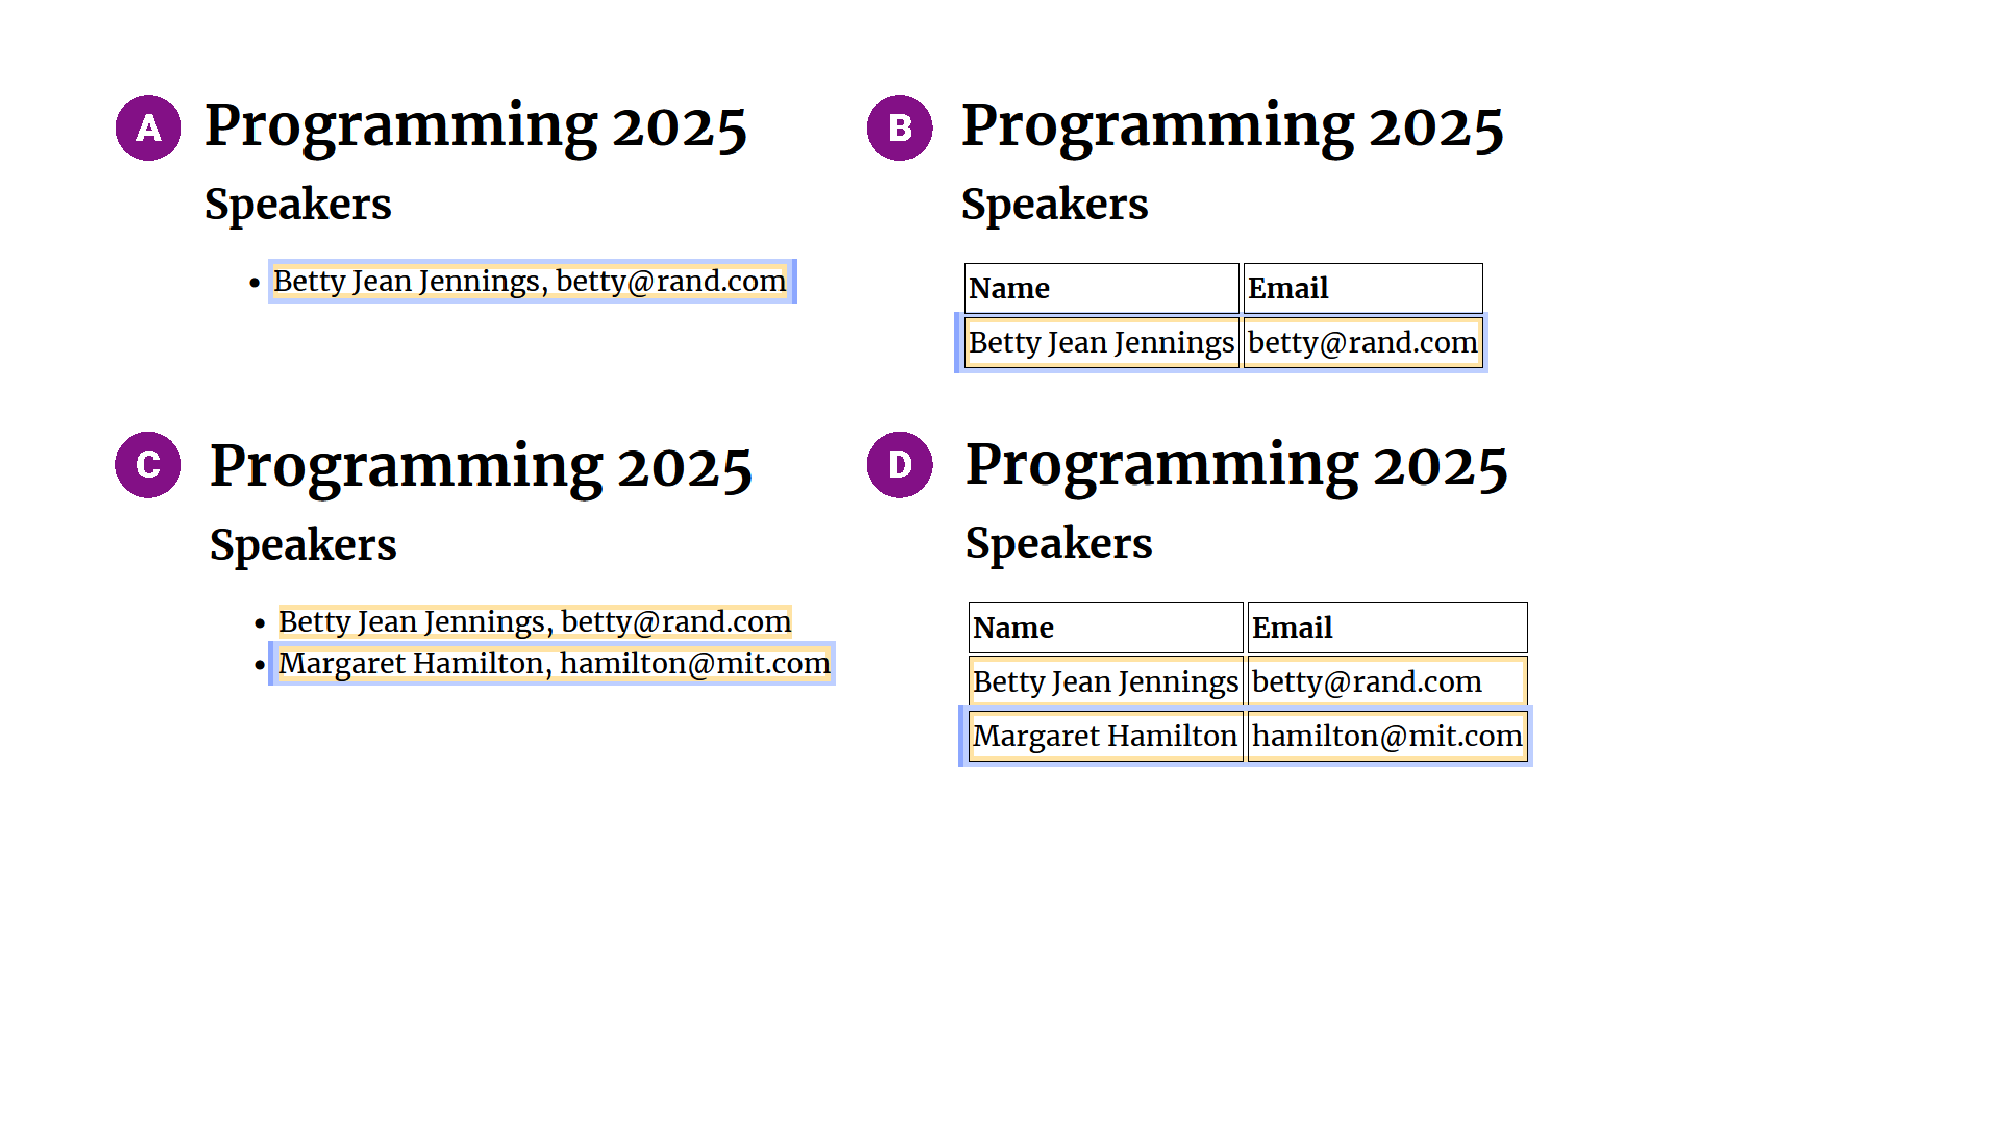
\includegraphics[width=0.95\columnwidth,clip,trim=1.7cm 6cm 7.8cm 1.5cm]{fig/merging.pdf}
\caption{Merging of two independently done sequences of edits. Two ways of merging B and C result in the same D.}
\label{fig:merging}
\end{figure}

% --------------------------------------------------------------------------------------------------

\section{Programming Experiences}
\label{sec:impl}

The key claim of this paper is that the Denicek computational substrate makes it easy to support
a range of compelling user experiences. The experiences can be implemented by composing the
primitive operations of the substrate, relying in particular on the operation for merging edits.
We demonstrate this claim with the web-based Webnicek system, which uses Denicek to support:
%
\begin{enumerate}[itemsep=0pt,label=(\roman*),topsep=3pt,leftmargin=20pt]
\item collaborative document editing (\S\ref{sec:impl-collab}),
\item programming by demonstration (\S\ref{sec:impl-pbd} and \S\ref{sec:impl-interaction}),
\item incremental recomputation (\S\ref{sec:impl-eval} and \S\ref{sec:impl-incremental}),
\item schema change control (\S\ref{sec:impl-schema}),
\item end-user debugging via provenance tracking (\S\ref{sec:impl-provenance}),
\item concrete programming via managed copy \& paste (\S\ref{sec:impl-copy}).
\end{enumerate}
%
We describe the programming experiences in isolation in the context of Webnicek in this section.
The data science notebook system Datnicek, discussed in \S\ref{sec:case}, provides
a more comprehensive case study by combining multiple user experiences together.

\subsection{Collaborative Editing}
\label{sec:impl-collab}

Denicek enables collaborative editing as illustrated earlier (\S\ref{sec:walk}, E).
If a document is edited by multiple users, they can each make edits to their local copy and
eventually merge the variants using the operation to reconcile edit histories. Merging requires
coordination among users, but not a central server as in local-first software~\cite{kleppmann-2019-local}.

Merging of histories behaves akin to git rebase in that it keeps a linear history. Synchronization
in a distributed system thus requires first reapplying local edits on top of the remote history,
before updating the remote history. Denicek thus implements the \emph{convergence model} of
document variants \cite{edwards-2025-schema}, i.e., the user cannot, for example, maintain their
own local document structure and import new data from another variant (an alternative discussed
in \S\ref{sec:discuss}).

Consider the scenario in Fig.~\ref{fig:merging}. Here, the document $D$ can be obtained
either by appending $C'$ (produced by the edit reconciliation operation) on top of $A,B$ or by
appending $B'$ on top of $A,C$. The edit histories resulting from the two ways of merging will
differ. In the first case ($B$ then $C'$), the \ident{Append} edit that adds a new node is followed
by further focused edits that transform the newly added node from a list item to a table row.
In the second case ($C$ then $B'$), the structural transformations are applied to all rows.

According to the current implementation of our effect analysis, the two example histories are conflicting.
Although $B$ primarily affects the document structure, it also adds a new field to the record (email),
which is a \ident{ValueEffect}, conflicting with the \ident{ValueEffect} of $C$. In this scenario, the
conflict can be ignored and the resulting document will be the same.  However, as discussed
in \S\ref{sec:system-ops}, merging of edit histories is not symmetric and arising conflicts
can also be resolved by removing conflicting edits.

% \note{To guarantee that replicas converge it is necessary to have a global order on merges.
% OT and CRDT algorithms use timestamps combined with a unique ID for each client to establish
% this global order without a centralized coordinator. We can do the same. This means you never
% know if your changes will dominate or whether they will be eventually overriden but people
% seem to be willing to live with it. Personally, I'm a skeptical: I expect that like with NoSQL
% people will eventually realize this sucks and go back to centralized systems.}

% --------------------------------------------------------------------------------------------------

\begin{figure}[t]
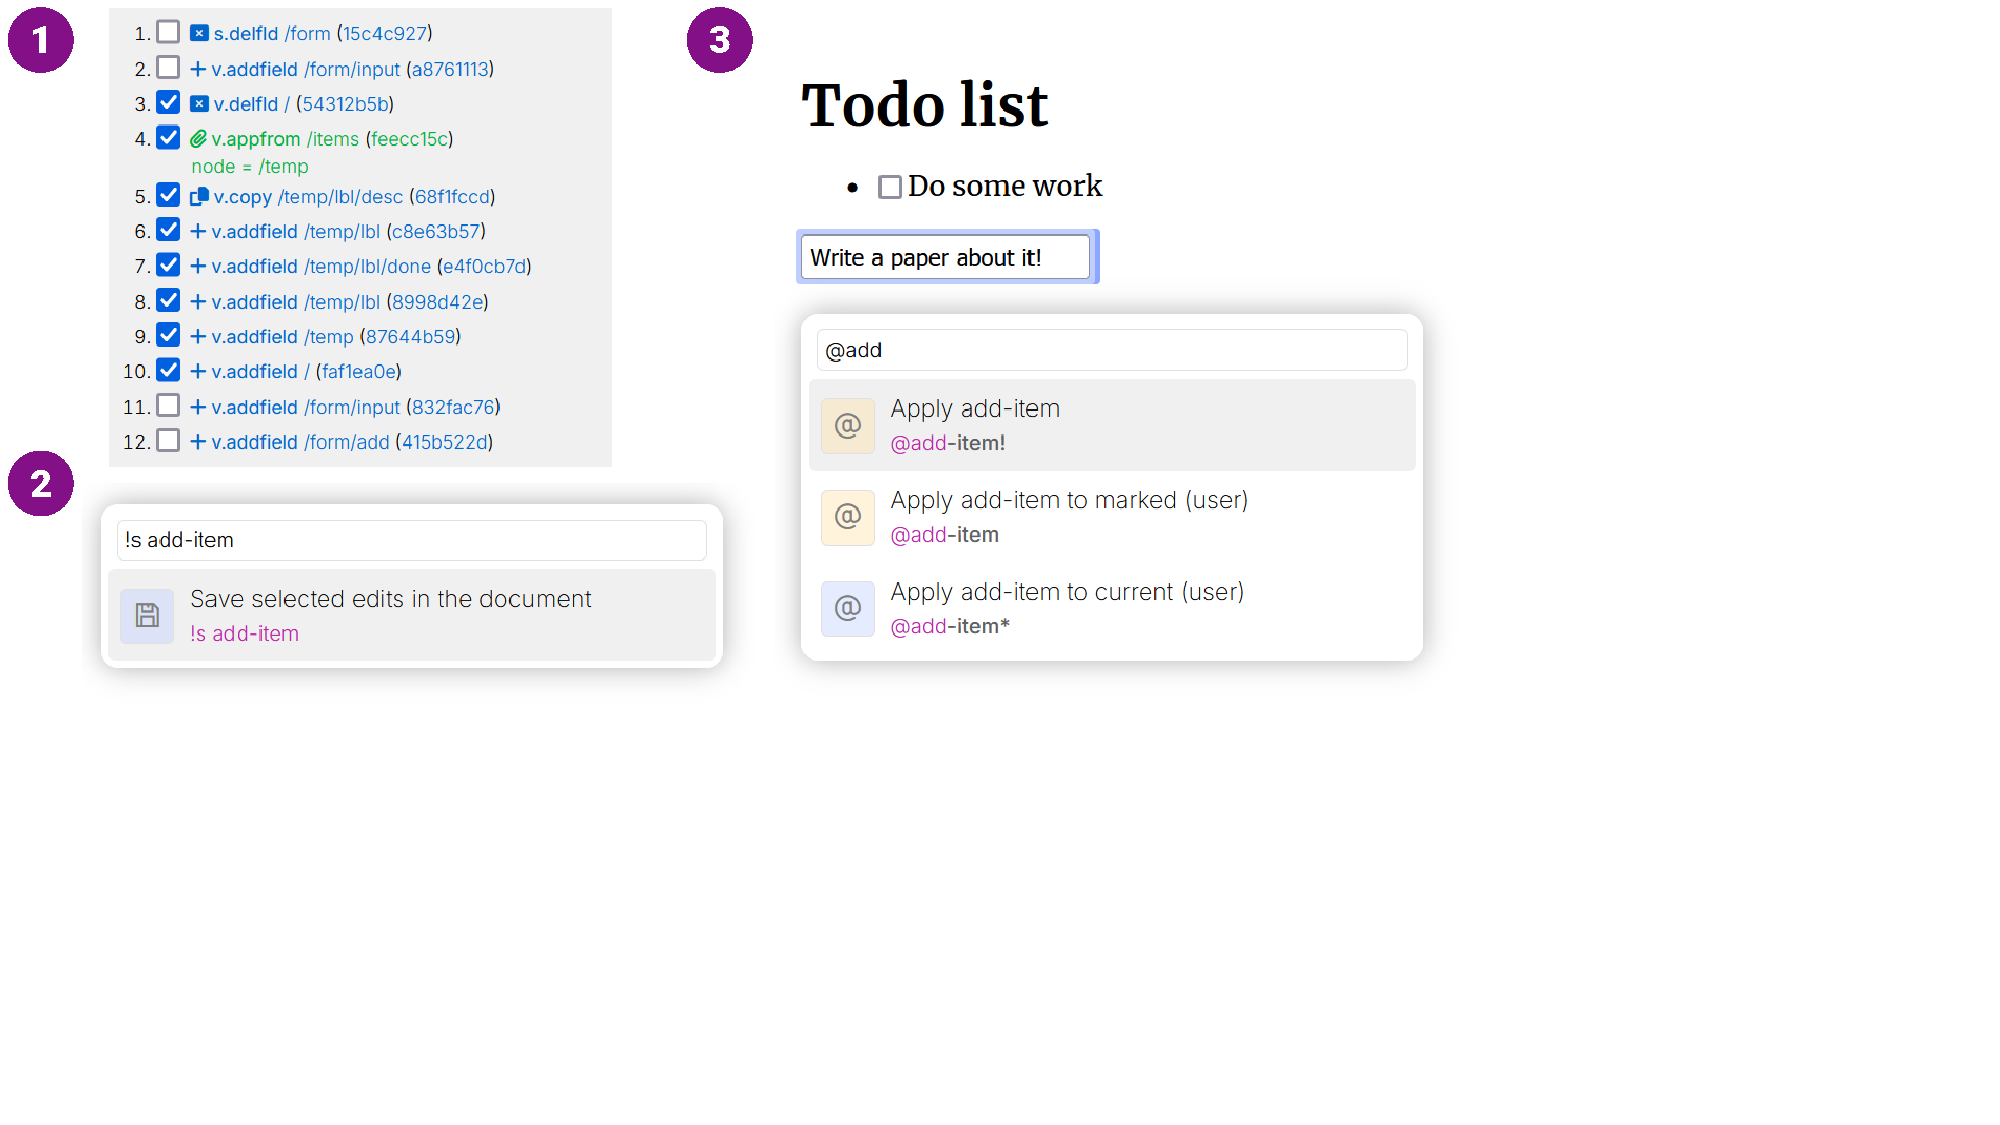
\includegraphics[width=0.9\columnwidth,clip,trim=0cm 7cm 9cm 0cm]{fig/pbd.pdf}
\caption{Programming by demonstration is implemented by selecting edits from the document
history (1), saving them in the document (2) and replaying them (3).}
\label{fig:pbd}
\end{figure}

% --------------------------------------------------------------------------------------------------

\subsection{Programming By Demonstration}
\label{sec:impl-pbd}

In programming by demonstration \cite{cypher-1993-pbd}, the user demonstrates a task to the
system and the system then repeats it, directly or in a generalized way. To use direct
repetition with Denicek (Fig.~\ref{fig:pbd}), the user selects edits from the edit history,
names them and replays them. For general-purpose document editing in Webnicek, this requires
certain forethought, but as shown in \S\ref{sec:case}, the mechanism is very effective
in a domain such as data wrangling \cite{kandel-2011-wrangler}.

There are two notable aspects of our implementation of programming by demonstration in Webnicek.
First, Webnicek records the saved edits in the document itself (by representing individual edits
as nodes and storing them in a list inside the {\small\Verb_/saved-interactions_} field).
This means that no other implementation mechanism outside of Denicek is needed and also
that the stored edits can be modified by the user or tools working with the document.

Second, when replaying edits, Webnicek does not append the recorded edits on top of the current
history. Instead, it stores the hash of the history at the time of saving. To replay the edits,
it then appends the edits to the top of the original history and merges this edit sequence
with the current history. This pushes the recorded edits through later edits made by the user,
reconciling them with potential structural edits. The result can be seen in Fig.~\ref{fig:walkthrough} (E), where
a newly added list item becomes a table row.

Webnicek also accounts for the case where edits recorded in the document are themselves
transformed (when they are reconciled with other edits during merging). In this case, Webnicek
updates the recorded edits (an alternative approach is discussed in \S\ref{sec:discuss}).

% Simply replaying recorded edits provides limited programming capabilities. We discuss in the
% next section how recorded edits can themselves be edited by the user to generalize and
% conditionalize their effects. More general and conventional programming constructs are discussed in \S\ref{sec:discuss}.

% --------------------------------------------------------------------------------------------------

\begin{figure}[t]
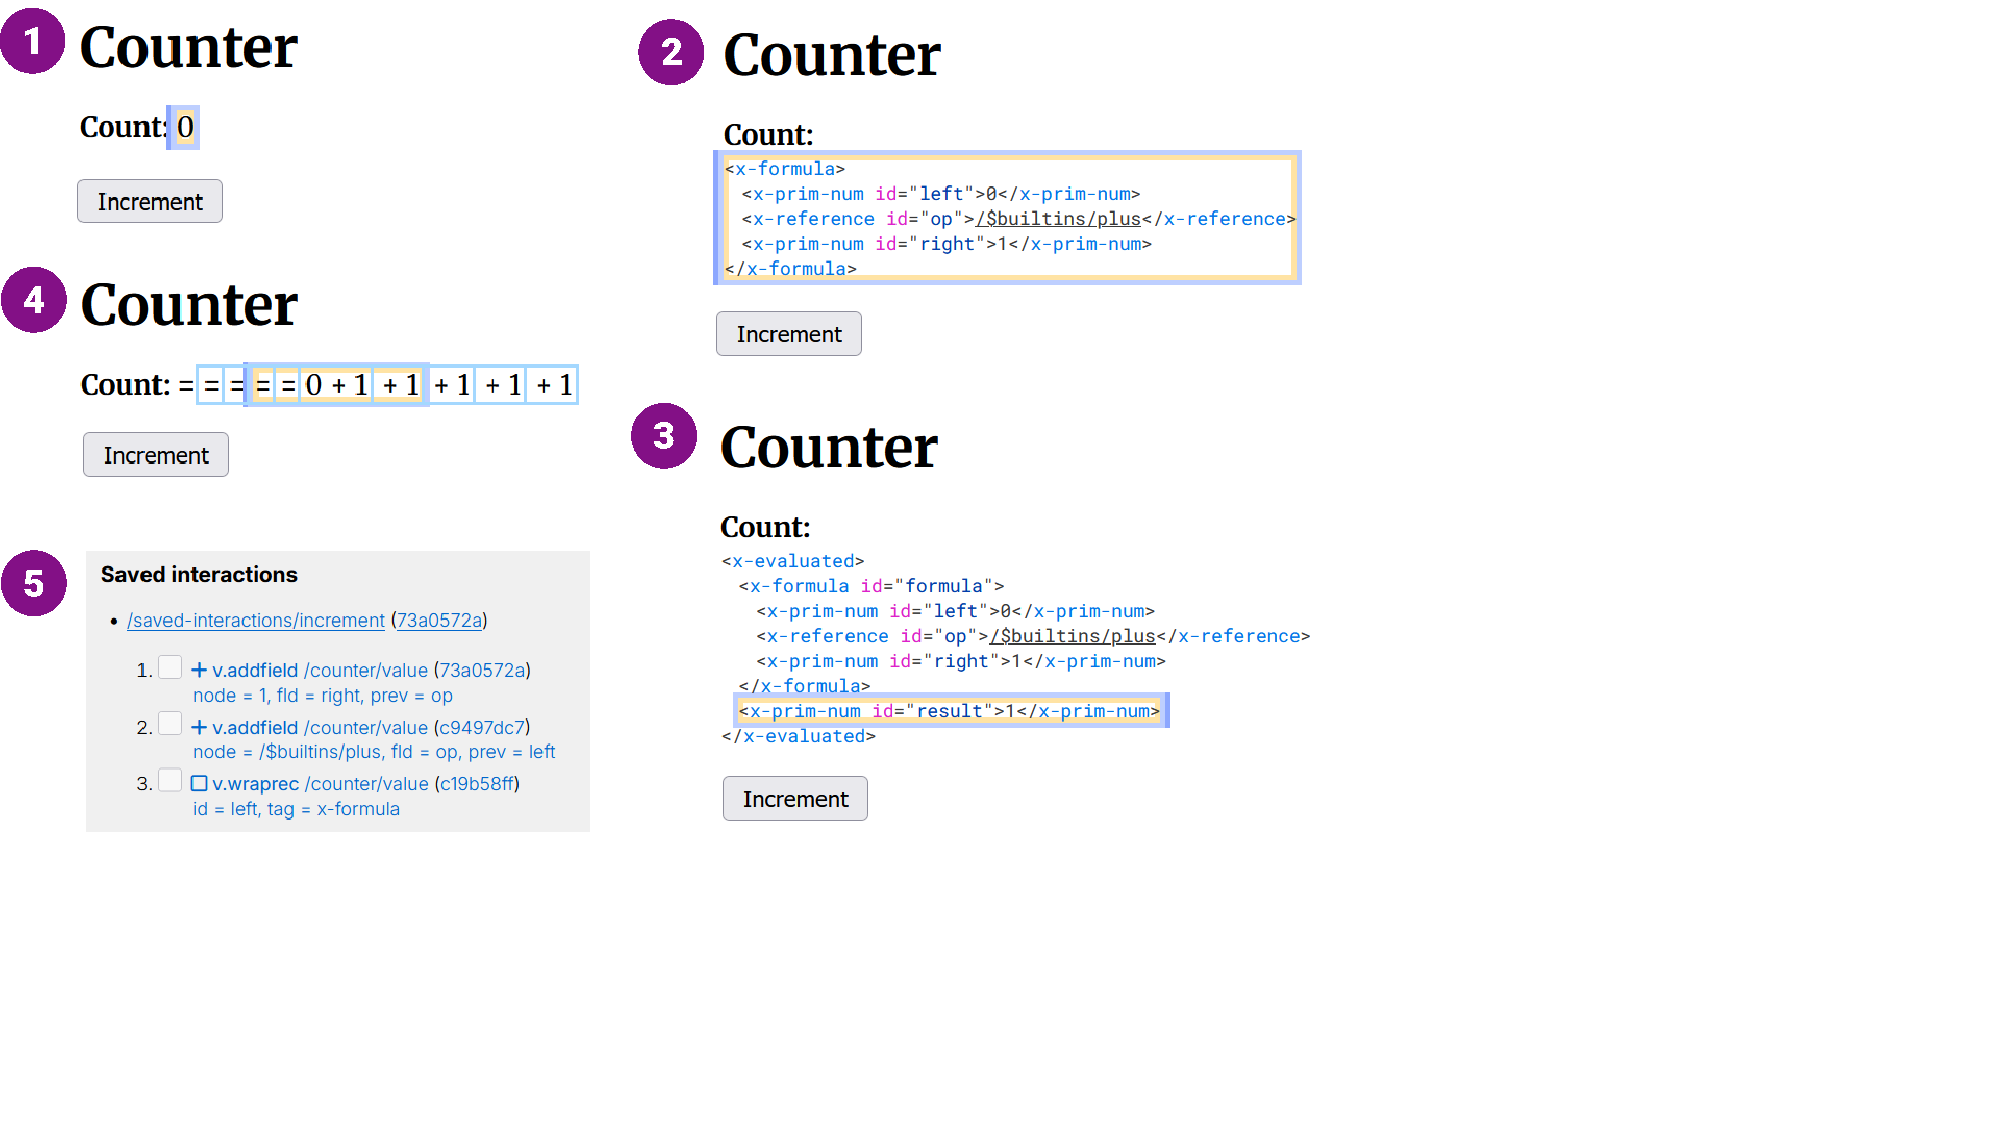
\includegraphics[width=0.95\columnwidth,clip,trim=0cm 5cm 11.5cm 0cm]{fig/counter.pdf}
\caption{We wrap the initial count (1) in a formula that adds 1 to the
value, (2). Evaluation produces the count (3), which is invalidated on subsequent clicks (4).
The button replays the saved edits that wrap the current count in a formula~(5).}
\label{fig:counter}
\end{figure}

% --------------------------------------------------------------------------------------------------

\subsection{Interactive User Interfaces}
\label{sec:impl-interaction}

Programming by demonstration can be used to define interactive elements in the document. In a
simple scenario, illustrated in Fig.~\ref{fig:interactive}~(1), the {\small\Verb_click_} event
handler is set to a reference to a sequence of edits recorded in the document. Clicking the button
executes the edits using the mechanism discussed in the previous section, i.e., Webnicek appends
the edits to a history at the time when the edits were recorded and merges the edits with the
current history.

The use of merging when replaying recorded edits is crucial in both the Todo App and the Conference
List formative examples (see \S\ref{app:examples}). In both cases, the merging makes it possible to define
a user interface for adding items (new Todo items, new speakers) and later change the document
structure (refactor the speaker list into a table) or add functionality (formula to evaluate whether a
Todo item has been completed) without having to recreate the user interface for adding items.
The use of merging ensures that new items are added in a correct format or with the additional
functionality.

In addition to the core functionality provided by Denicek, the Webnicek system also makes it possible
to generalize the interactions recorded through programming by demonstration. As shown
in Fig.~\ref{fig:interactive}~(2), a button to remove all completed Todo items can be created by
generalising the {\small\Verb_remove-item_} interaction, which removes the list item at the index 0.
In addition to the recorded interaction, we manually specify (in the source view) that the edits
should be applied to all elements selected by the {\small\Verb_/items/*_} selector, instead of
the original {\small\Verb_/items/0_} selector (prefix) and that the edits should only be
applied to elements for which the formula (which tests if the checkbox is checked) specified by a
relative selector {\small\Verb_./condition/comp/result_} evaluates to true.

Note that the generalization mechanism does not violate the Denicek principle that edits cannot
depend on values (\S\ref{sec:system-defs}). Webnicek finds all nodes for which the condition
holds and generates one specific (non-conditional) edit for each of the nodes.

% \note{The above paragraph was surprising to me and I'm not sure I fully understand it even after
% staring at the figure for a while. Edits are recorded as an AST using x-tags to hide them
% in the UI? That became clear only after reading the next section. Our audience might be a lot
% happier if we used a textual grammar. Earlier it was said that edits can't be conditional but
% then a conditional predicate appears here. This is a special feature of button nodes? Or event
% handler nodes? This starts to resemble Angular and similar template languages (which I find hard to read).}
%
% TP: Haha, Angualr - oh no! But I don't have a better solution right now sadly...

\keyideabox{\faMagic}{Generalization Heuristic}{Specifying generalization manually is cumbersome.
Programming by demonstration systems typically implement heuristics for generalization
\cite{myers-2000-intelligence} that infers and suggests such generalizations. If integrated into
Webnicek, such heuristic could for example automatically construct a formula
based on positive and negative examples \cite{gulwani-2014-flash} (selected and deselected Todo
list items).}

% --------------------------------------------------------------------------------------------------

\begin{figure}[t]
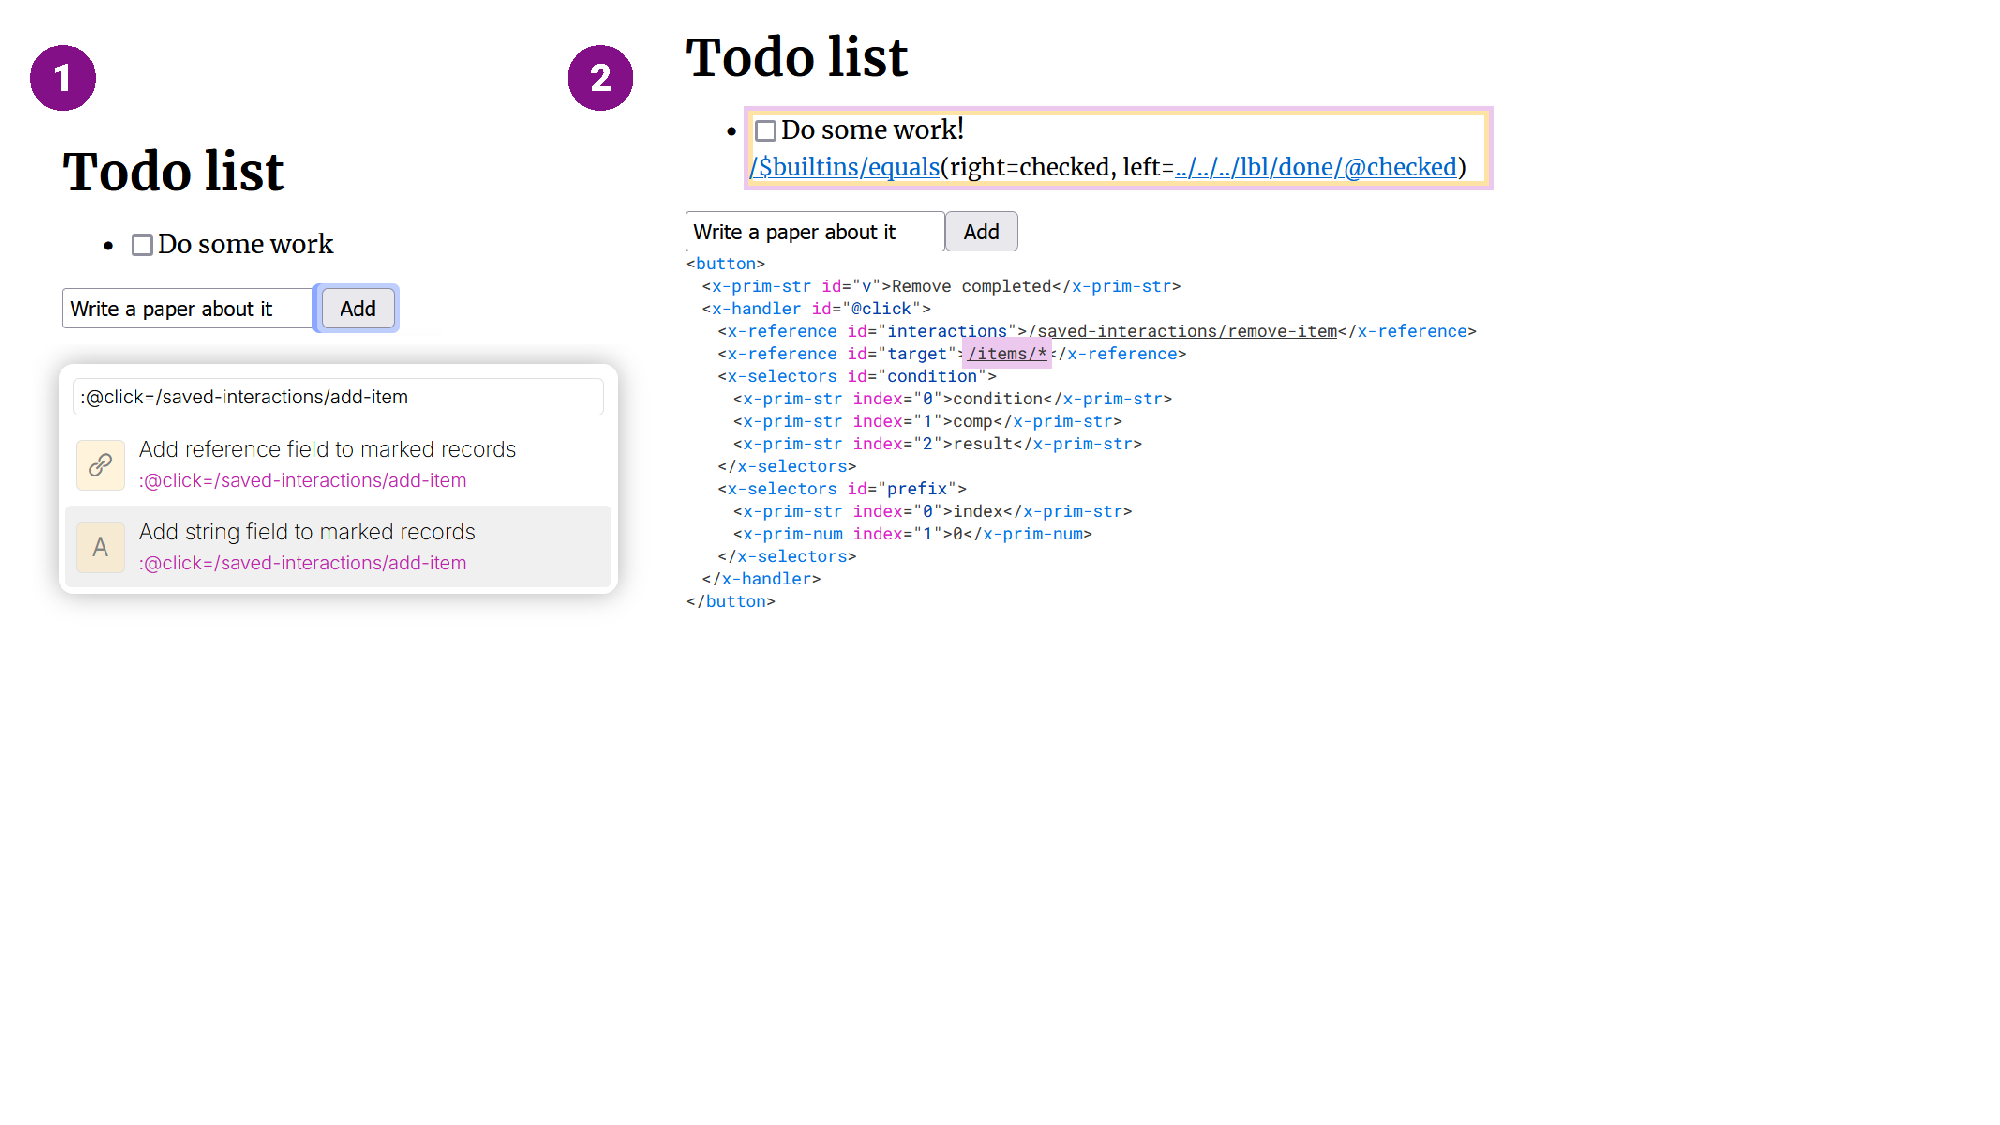
\includegraphics[width=1\columnwidth,clip,trim=0.5cm 8.5cm 8.5cm 0.5cm]{fig/interactive.pdf}
\caption{Using programming by demonstration to define a UI. The ``Add'' button (1) replays edits;
the ``Remove completed'' button (2) modifies target and specifies a condition. }
\label{fig:interactive}
\end{figure}

% --------------------------------------------------------------------------------------------------

\subsection{Formula Language and Evaluation}
\label{sec:impl-eval}

As illustrated earlier (\S\ref{sec:walk}, F), Denicek documents can contain formulas inspired by the
spreadsheet paradigm \cite{nardi-1990-spreadsheets}. Formulas in Webnicek do not transform the
document and their results are transient, but they can describe richer computations than what can
be expressed using document edits.

Formula evaluation also leverages Denicek's ability to merge edit histories.
As illustrated in Fig.~\ref{fig:counter}, formulas are represented as document nodes with a
special tag ({\small\Verb_<x-formula>_}). They are recognized by a formula evaluator and
rendered in a special way (4), but they are created using ordinary
edits and the Denicek substrate treats them as standard nodes.

To evaluate formulas, the formula evaluator generates edits that turn the {\small\Verb_<x-formula>_} (2)
record into {\small\Verb_<x-evaluated>_} (3), which keeps the previous
formula state in the {\small\Verb_formula_} field and the evaluation result in the {\small\Verb_result_} field.
Keeping the previous state of the formula is not necessary, but it enables provenance analysis
as discussed in \S\ref{sec:impl-provenance}. The way edits generated by evaluation are merged
with the document is discussed in the next section.

% \note{As I've said before, I'd prefer to store the result of the formula inside the <x-formula>
% record instead of wrapping it on evaluation. This avoids changing the shape of the document on
% evaluation, which I recall added some complexity earlier.}
%
% TP: I think I tried that, but it still did not solve my problem - because I needed to add
% child nodes to the result. So this can probably only be done for a statically typed version.

The Counter App example shown in Fig.~\ref{fig:counter} illustrates the interaction between formulas
and programming by demonstration. To implement a counter, we first add the initial value 0 to the
document. We then perform three edits that wrap the current counter value in a formula that adds
1 to the value. The three edits (5) are used as an event handler for the button and so clicking the
button creates an increasingly long sequence of increments. One advantage of this approach that
we will leverage later is that the evaluation also records a trace of how the final computed value
was obtained.

% \note{OK maybe I'm finally getting it. You aren't mutating the value of the counter, you're wrapping
% the value in an increment formula. I never got that in our previous discussions. Presumably that
% evaluation is now frozen so it serves as an execution trace. This is a lot different from my
% approach where a formula stays unchanged except for the results. One advantage is that fields
% contain a record of their computed mutations whereas in my approach that is recorded in the
% past state of the doc whence the mutation occured.}

\keyideabox{\faSuperscript}{Formula Language}{
Webnicek exposes the underlying representation of formulas to the user, but the same representation
could be edited through a user-friendly mechanism such as a textual calculation view \cite{sarkar-2018-calc},
or a block-based editor \cite{jansen-2019-xlblocks}. The key point
is that Denicek's tree structure makes it easy to embed formulas in document in a uniform
way, edit them as other nodes and merge edits that change them.}

% --------------------------------------------------------------------------------------------------

\subsection{Incremental Recomputation}
\label{sec:impl-incremental}

As illustrated in Fig.~\ref{fig:incremental}, Webnicek supports incremental recomputation.
The cost of speaker travel depends on the number of speakers, but the cost of refreshments
depends only on two constants. The edit that adds a speaker invalidates only the former computation.

The evaluation mechanism is illustrated in Fig.~\ref{fig:eval}. When the formulas are evaluated,
Denicek generates edits that wrap the formula in {\small\Verb_<x-evaluated>_} and set the result
to the computed value. In Webnicek, those evaluated edits are kept in a separate list that is always
appended to the top of the current edit history. When the user makes subsequent edits, the evaluated
edits are pushed through the newly added edits using edit reconciliation. If the edits conflict
(according to the conflict detection discussed in \S\ref{sec:system-ops}), the affected evaluated
edits are dropped.

The dependencies between edits alongside with the conflict detection mechanism provide functionality
that other systems implement using an explicit dependency graph or by topological sorting.

\keyideabox{\faRefresh}{Live Programming}{The Webnicek prototype does not automatically
evaluate formulas. This makes it easier to understand the evaluation
mechanism, but a realistic system based on the substrate could automatically evaluate
formulas to provide a live programming experience \cite{petricek-2020-live,rein-2019-live}
and use incremental recomputation for performance~reasons.}

% \note{I'm confused. Changing the value of a location conflicts with an edit that evaluates a
% formula containing a reference to that location? And these evaluation edits are second-class
% edits that get retroactively dropped to ``unevaluate'' the formula? I'd prefer what you suggest
% above: formulas are seemingly globally re-evaluated after every change, with incremental
% computation a hidden perf optimization. }

% \note{An important property of incremental computation systems is avoiding redundant execution.
% Usually this involves a topological sort of the computation dependency graph. We may need to
% have a story about that to avoid hate from reviewer 2. Personally, I think incremental
% recomputation is about performance, not the programming experience, so it isn't that important for this paper. }
%
% TP: The cool thing is we get this for free! Clarified.


% --------------------------------------------------------------------------------------------------

\begin{figure}[t]
  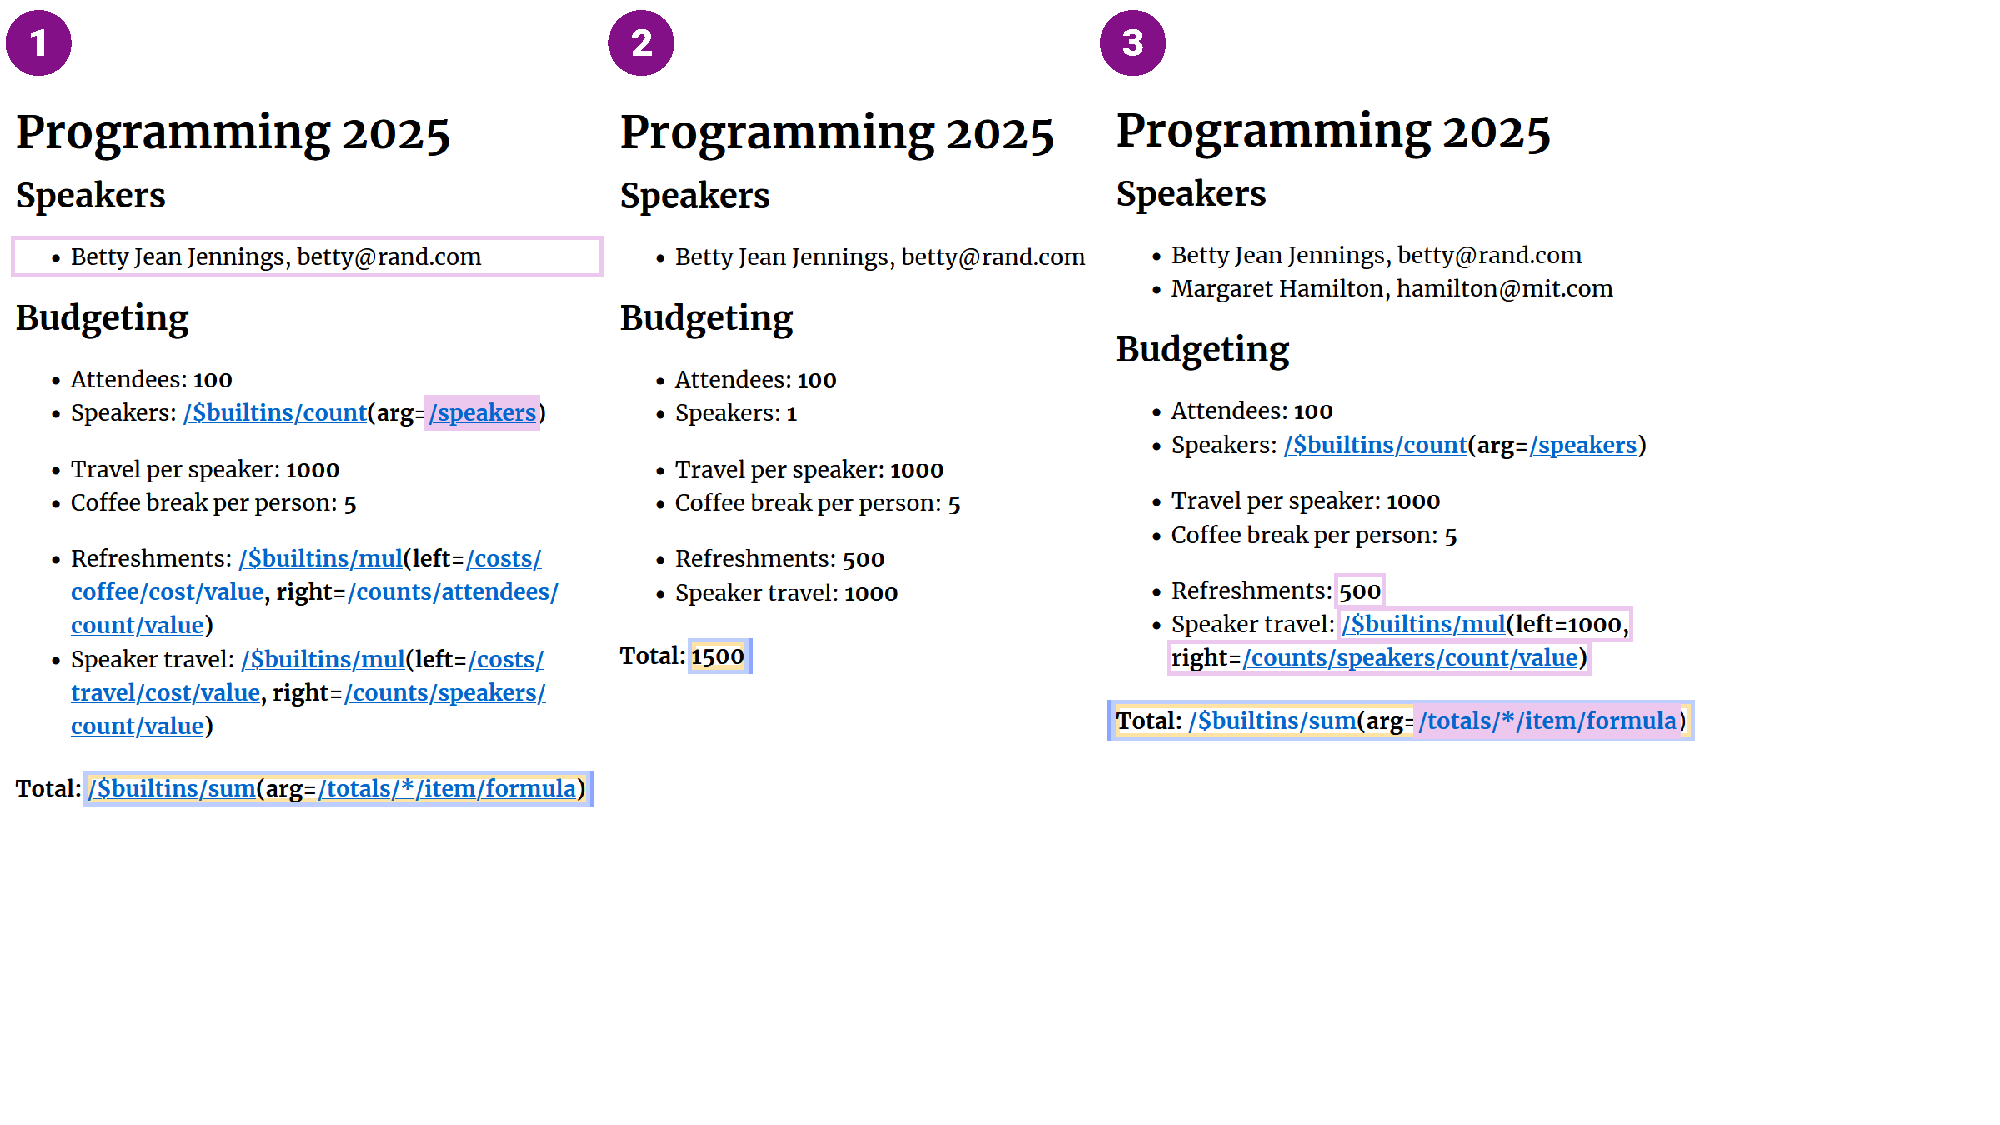
\includegraphics[width=1\columnwidth,clip,trim=0.1cm 5cm 5.1cm 0cm]{fig/incremental.pdf}
  \caption{Budget calculation based on the number of speakers (1) and the result (2). When speaker
  is added (3), only the results of affected formulas are invalidated.}
  \label{fig:incremental}
  \vspace{-1em}
\end{figure}


% --------------------------------------------------------------------------------------------------

\begin{figure}[h]
\centering
\begin{minipage}{0.55\columnwidth}
  ~\\[1em]
  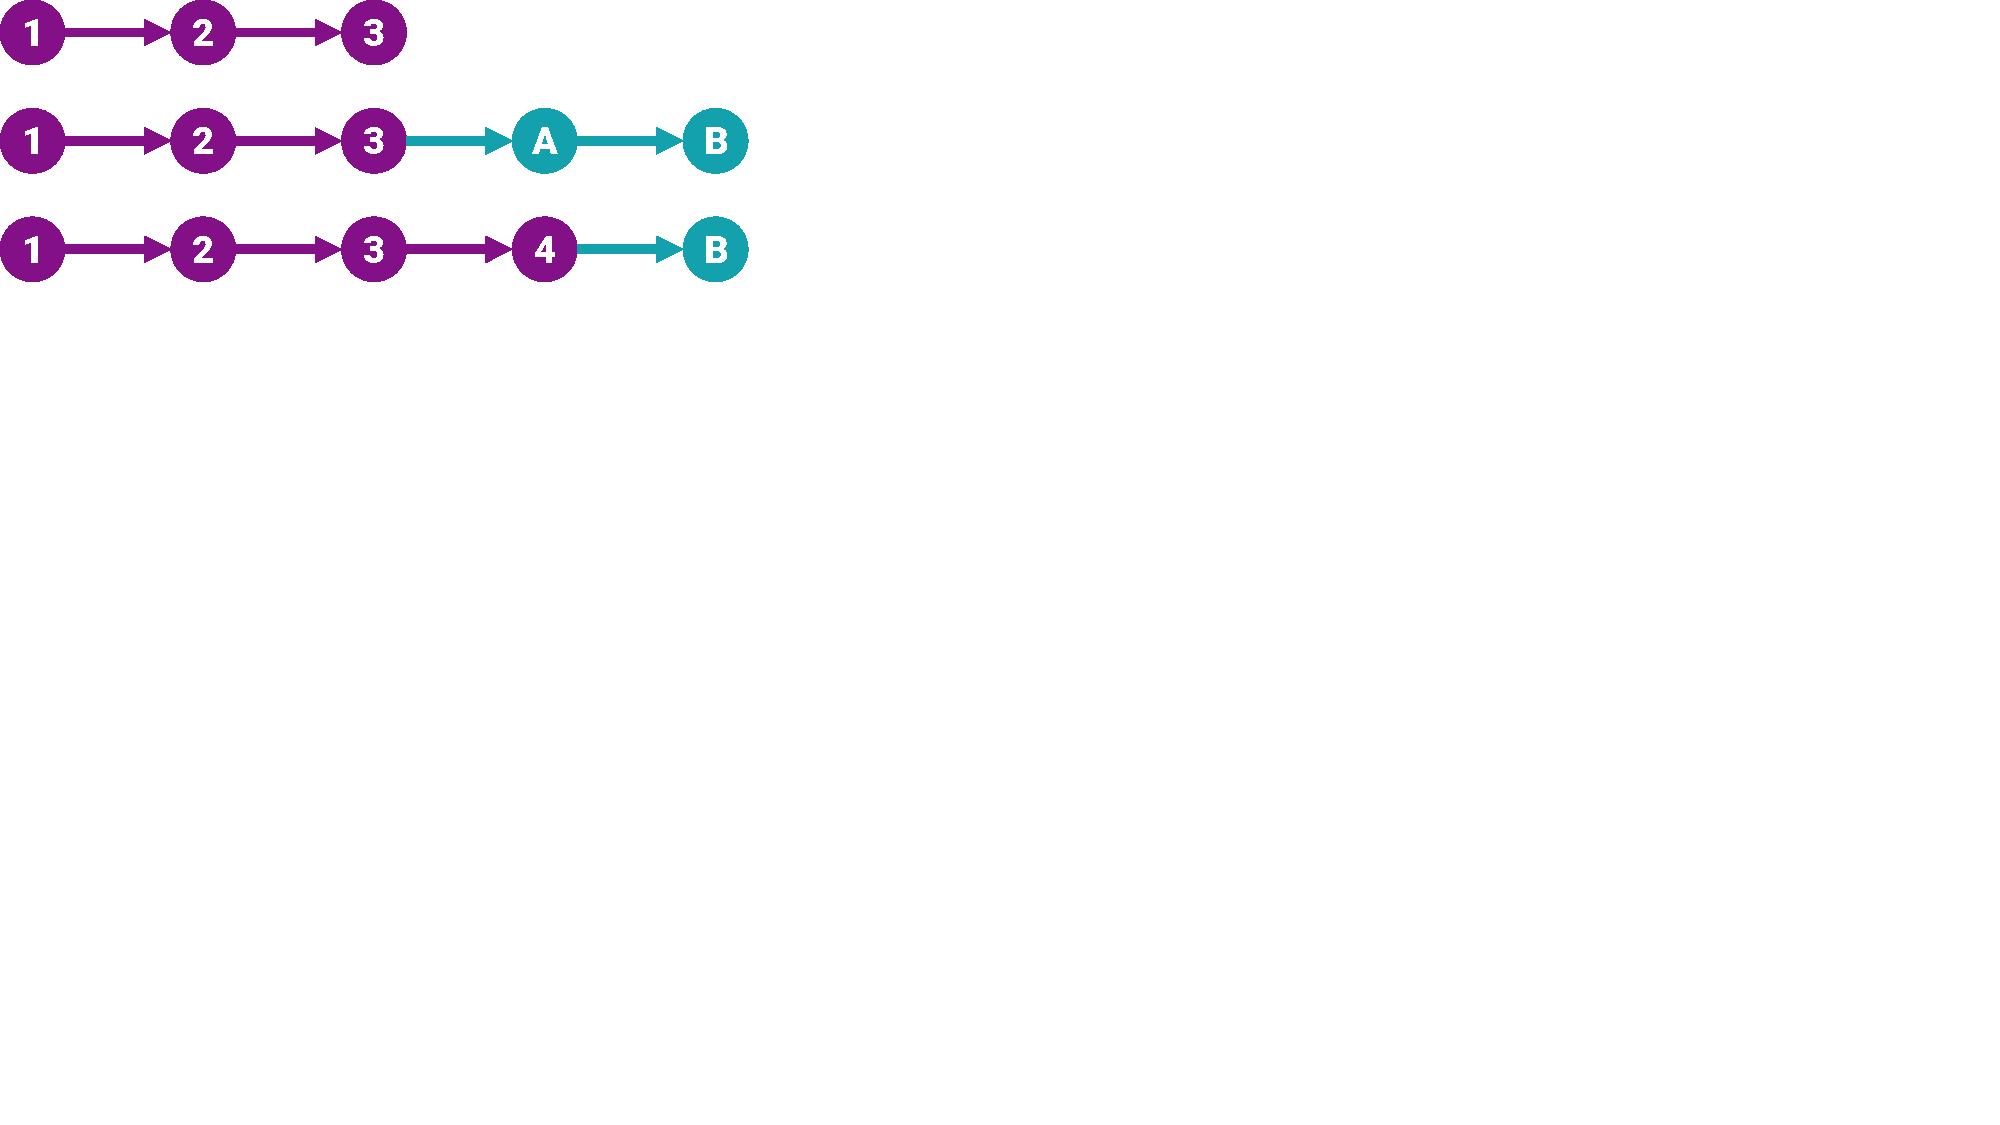
\includegraphics[width=0.9\columnwidth,clip,trim=0cm 14cm 21cm 0cm]{fig/eval.pdf}
  \end{minipage}%
  \begin{minipage}{0.45\columnwidth}
    \caption{Evaluated edits (A, B) are kept at the top of the history. Evaluated edits (A)
      that conflict with ordinary edits (4) are dropped.}
    \label{fig:eval}
  \end{minipage}
\end{figure}

% --------------------------------------------------------------------------------------------------

\subsection{Schema Change Control}
\label{sec:impl-schema}

Document structure often needs to evolve \cite{burnett-2014-silos}, as illustrated by the formative
example Conference List where a list is transformed into a table. When this happens,
data and code that depend on the structure of the document need to evolve correspondingly.
The problem is well-known in database systems \cite{rahm-2006-schema} and has recently been
explored in the context of programming systems \cite{edwards-2025-schema}.

Although Denicek does not explicitly track document structure (schema or type), all documents
have an implicit structure and some edits transform this structure. As
discussed in \S\ref{sec:system-ops}, Denicek automatically updates reference nodes in the
document when edits modify the document structure. This enables a form of schema and code
co-evolution \cite{edwards-2025-schema}. Formulas embedded in documents use reference
nodes to refer to both data sources (in the document) and the results of other computations.
Consequently, if the document structure changes, the formulas are automatically updated.

Consider the example in Fig.~\ref{fig:coevolution}. The original list {\small\Verb_<ul>_} is
turned into {\small\Verb_<tbody>_} using \ident{UpdateTag} and wrapped inside {\small\Verb_<table>_}
with a field {\small\Verb_body_} using \ident{WrapRecord}. For the latter, Denicek updates the
reference accordingly turning the original {\small\Verb_/speaker_} reference in the formula
into {\small\Verb_/speaker/body_}.

\diff{Note that Denicek can only reflect schema changes explicitly represented by the document
structure. If a formula depended on the structure of the original string representing speakers
(with a comma), Denicek would not be able to amend the logic of the formula. Systems supporting
the divergence model \cite{edwards-2025-schema} may be able to lift this restriction by
transforming the new value back before applying the original formula.}
\note{Added response to R3's question about schema change}

Edits produced by document evaluation transform the formula structure (wrapping it in the
{\small\Verb_<x-evaluated>_} record). However, the reference behaviour of those edits is set
to keep references unchanged (as discussed in \S\ref{sec:system-defs}) and so references to
formulas are not transformed when the formula is evaluated (otherwise, references
would be updated to point to the original unevaluated formulas).

% --------------------------------------------------------------------------------------------------

\begin{figure}[h]
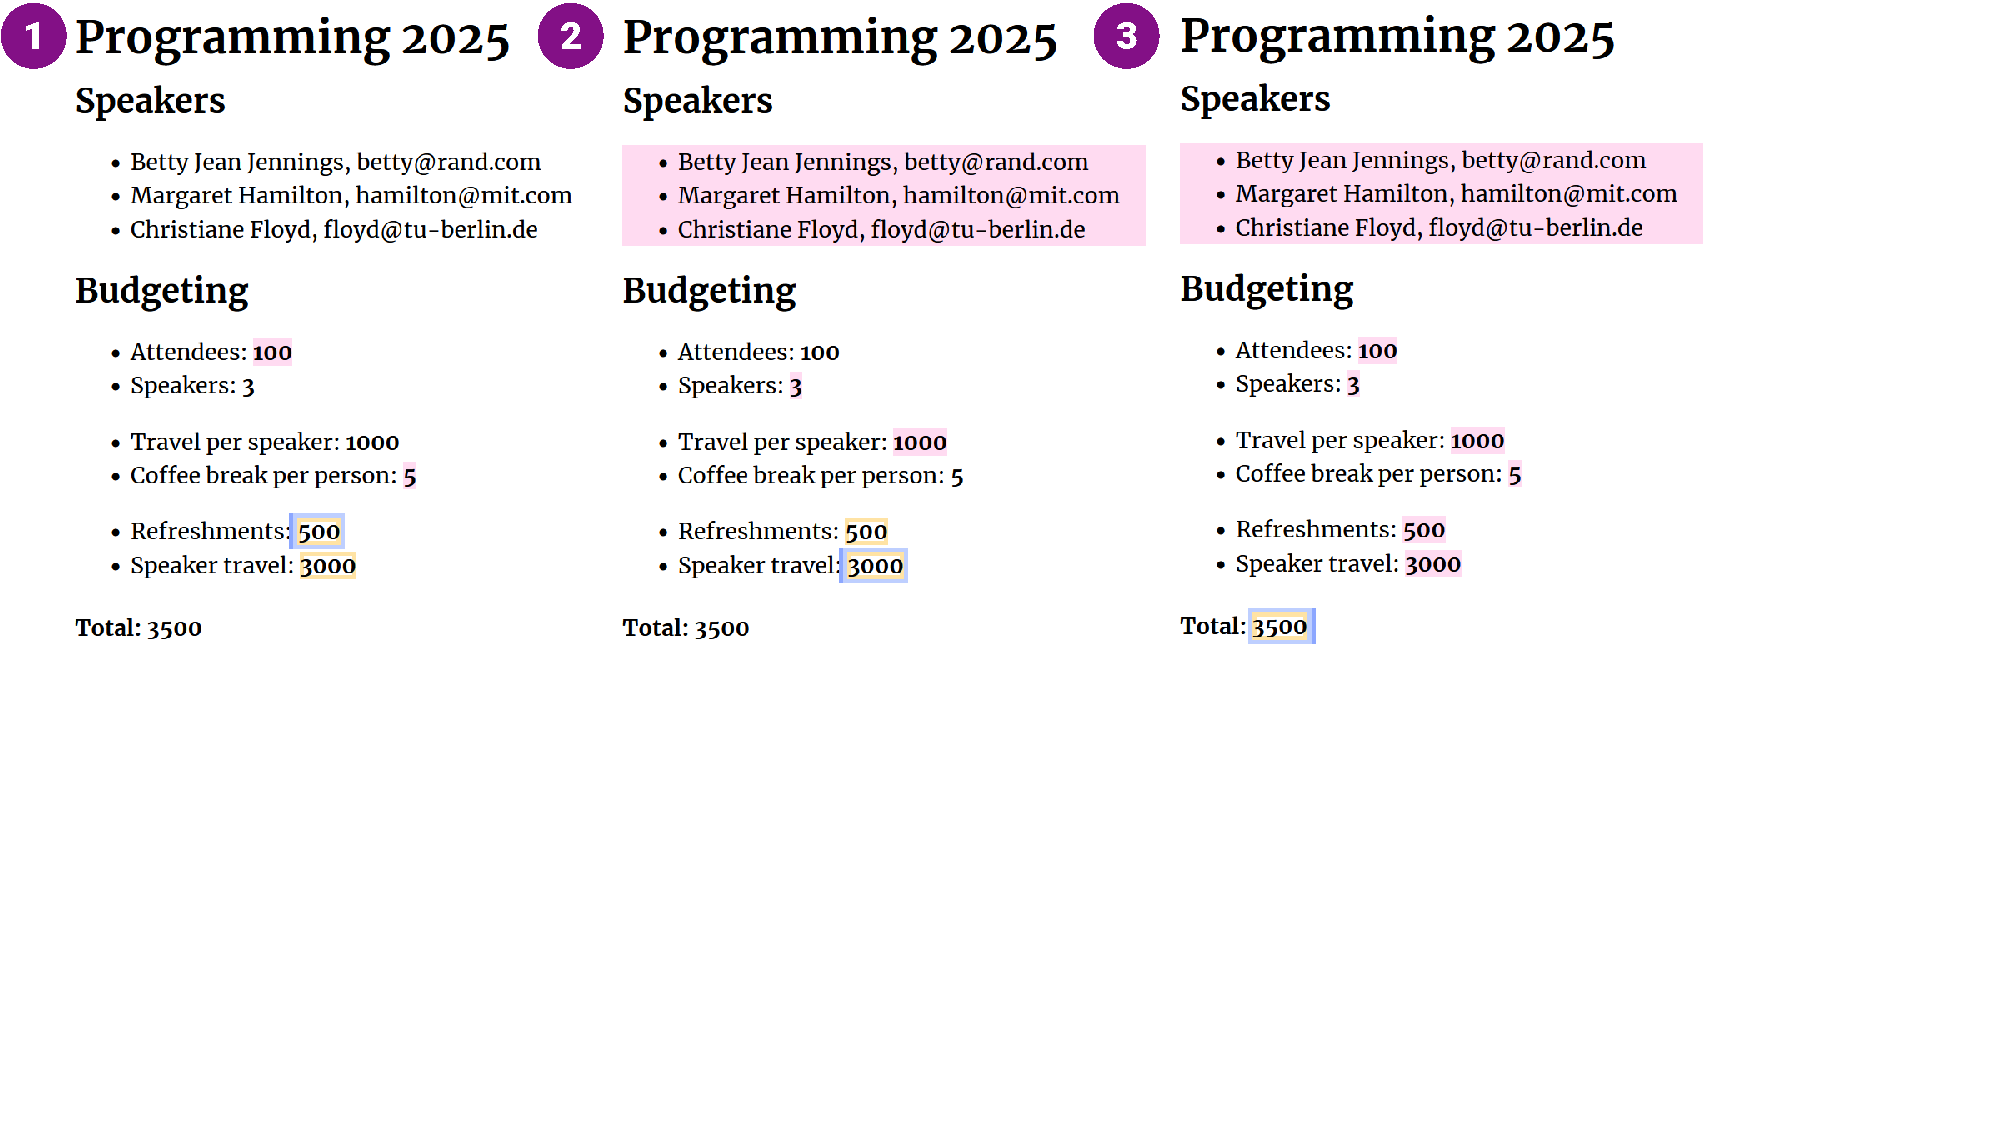
\includegraphics[width=1\columnwidth,clip,trim=0cm 8cm 5cm 0cm]{fig/provenance.pdf}
\vspace{-1em}
\caption{Using provenance tracking to highlight document parts that contributed to the
calculation of refreshments costs (1), travel costs (2) and all costs (3).}
\label{fig:provenance}
\end{figure}

% --------------------------------------------------------------------------------------------------

\subsection{End-User Debugging}
\label{sec:impl-provenance}

The most common kind of end-user programming question is determining whether a value they observe
is right or wrong \cite{kissinger-2006-debugging}. One way to help users answer the question is
to provide an explanation how a value was obtained \cite{ko-2009-whyline}. Webnicek provides a basic
mechanism that highlights document nodes that contributed to a specific computed result,
illustrated in Figure~\ref{fig:provenance}.

The implementation leverages the fact that evaluation wraps the previous state of the formula
(\S\ref{sec:impl-eval}). When a formula is fully evaluated, the {\small\Verb_<x-evaluated>_}
document node contains the result, but also a sub-tree with the full evaluation trace
\cite{perera-2012-functional}. We analyse the trace, collect all reference nodes in the trace and
highlight all nodes referred to in the computation. Denicek makes this easy as we
can collect references directly nested in the formula node.

\keyideabox{\faBarChart}{Explanations and Linked Visualizations}{In Webnicek, we implement
provenance analysis to show inputs involved in computation, but information from the execution
trace collected by the Denicek substrate can also be used to provide a detailed
explanation~\cite{perera-2012-functional} or to automatically construct
a linked visualization~\cite{perera-2022-linked}.}

% --------------------------------------------------------------------------------------------------

\begin{figure}[t]
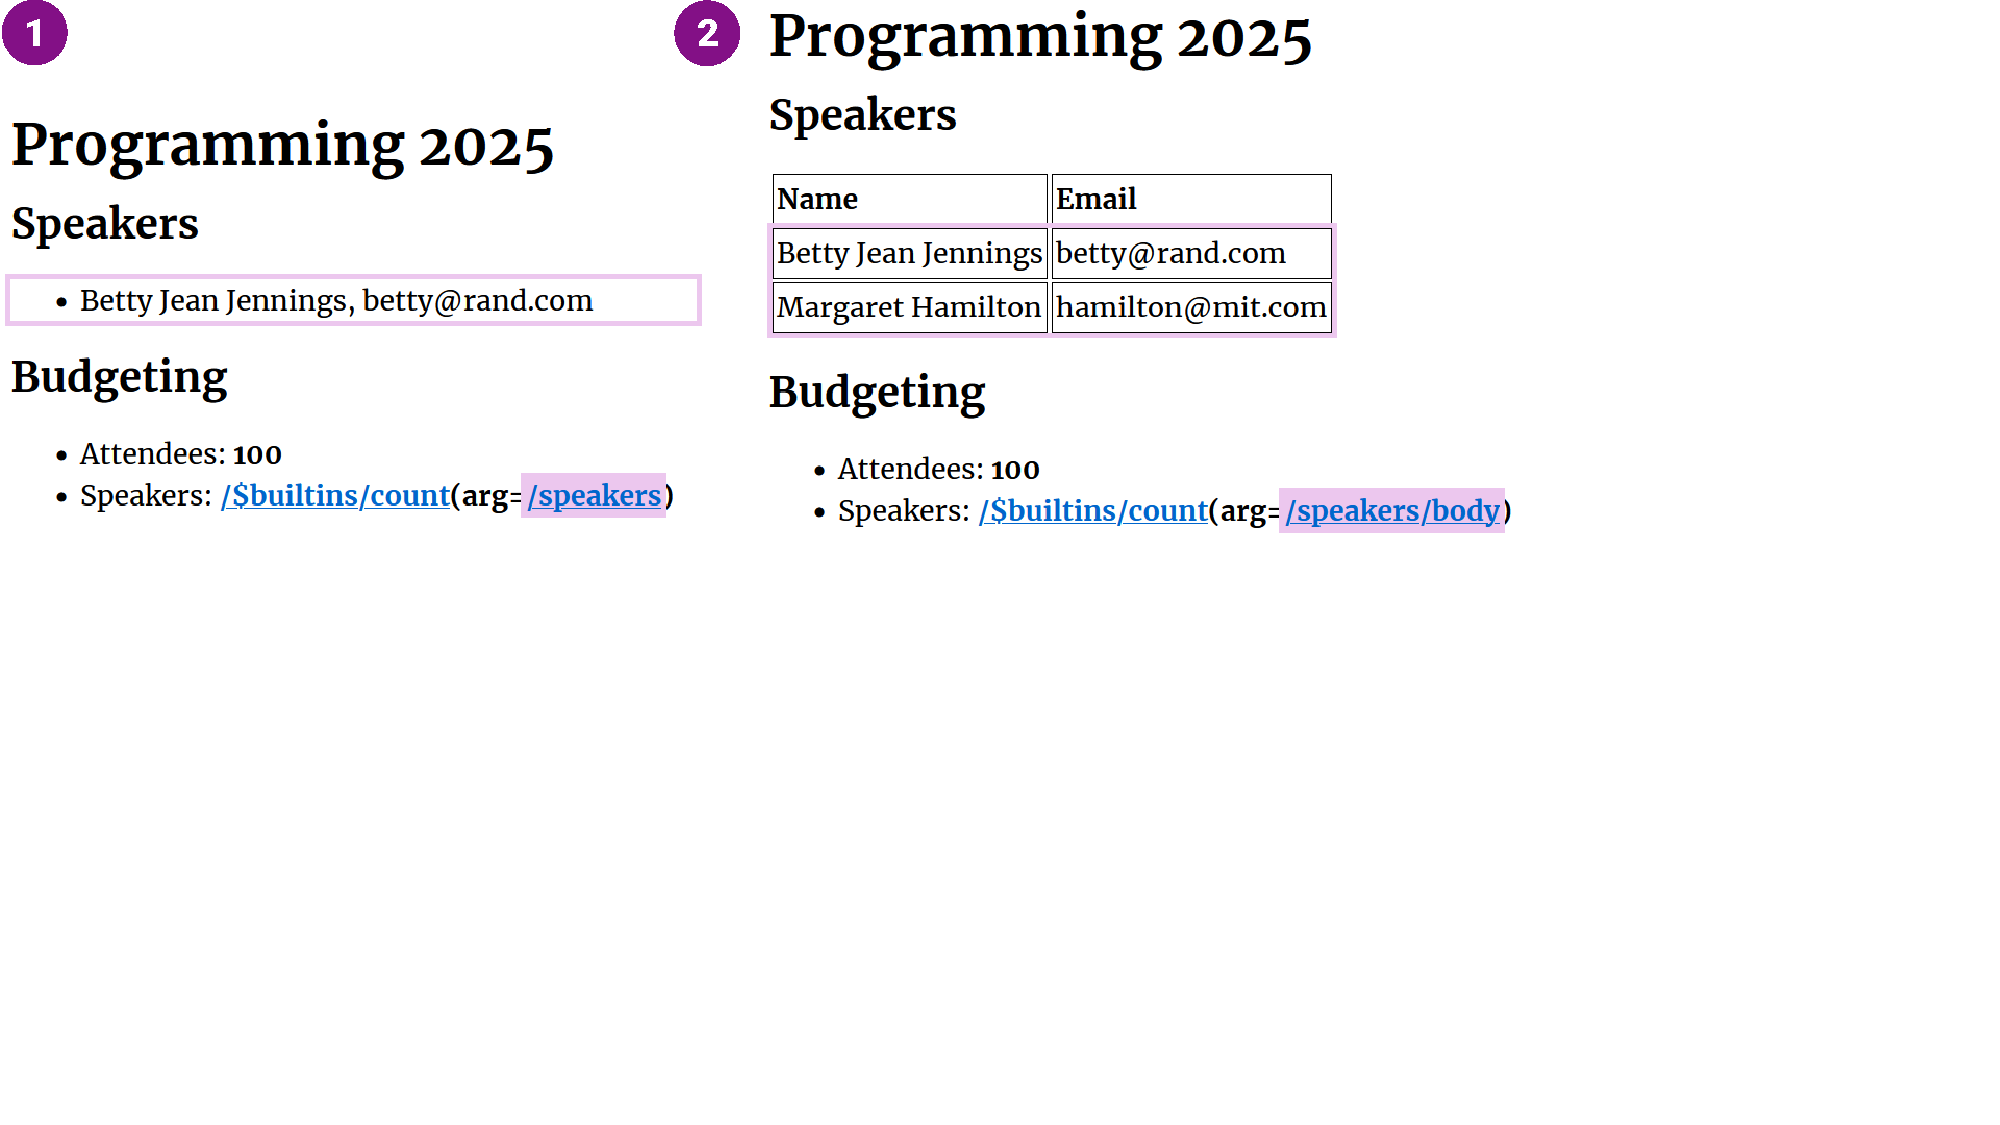
\includegraphics[width=0.9\columnwidth,clip,trim=0cm 9.5cm 8cm 0cm]{fig/coevolution.pdf}
\caption{When an edit changes the document structure, references in formulas are updated accordingly.}
\label{fig:coevolution}
\end{figure}


% --------------------------------------------------------------------------------------------------

\subsection{Concrete Programming}
\label{sec:impl-copy}

Abstraction is an essential feature of programming, but it has a high cognitive
cost~\cite{blackwell-2002-attention}. Programming by demonstration (\S\ref{sec:impl-pbd})
offers one way of reducing the cost. Another way is making programming more
concrete~\cite{edwards-2004-example,smith-1975-pygmalion}, i.e., to support copying of functionality
as in prototype-based object-oriented programming~\cite{ungar-1987-self,randall-1995-self}.

Webnicek supports a functionality akin to managed copy \&
paste~\cite{edwards-2006-copypaste,edwards-2022-copypaste} for formulas. Rather than introducing
abstractions (functions), users can copy and modify formulas to reuse them. When the user
discovers an error in the original formula, Webnicek lets them use the merging mechanism to correct
the error in the original formula and all its copies.

\note{Modified figure to add call to read-csv}
\diff{The functionality is illustrated in Fig.~\ref{fig:copypaste}, which uses the builtin operation}
{\small\Verb_read-csv_} \diff{to load a table from a file. The operation imports the data as a
document table with rows that can be addressed by subsequent formulas. The then user writes two
formulas to sum the rows and compute an average.}
\note{Add explanation of a more complex builtin operation}

They copy a formula with switched operands using
the \ident{Copy} edit and then modify it to use a different data source. They then navigate back
in history to the point before the copying and create a temporary fork of the document. In the
fork, they use \ident{RenameField} to switch the operands of the division. When they merge the
temporary fork into the original document, the \emph{Apply to Newly Added} logic of the merge
operation (\S\ref{sec:system-ops}) duplicates the \ident{RenameField} edits and applies them
to the copied formula. Merging with the \ident{Copy} edit and the fact that formulas
are ordinary document nodes, provide the key component for a straightforward implementation of the
managed copy \& paste functionality.

%\note{Nice and simple! My approach tried to be a lot fancier but ended up being too heavywieght. }

\keyideabox{\faClipboard}{Linked Editing}{Webnicek currently requires users to explicitly
manipulate history to correct errors across multiple code clones. Research on managing duplicated
code resulted in multiple tools \cite{toomim-2004-linked,duala-ekoko-2008-clone} with dedicated
user interface to manage clones. The Denicek substrate provides the underlying mechanism that
could be used to implement a more user-friendly interface inspired by those systems.}

% --------------------------------------------------------------------------------------------------

\begin{figure}[t]
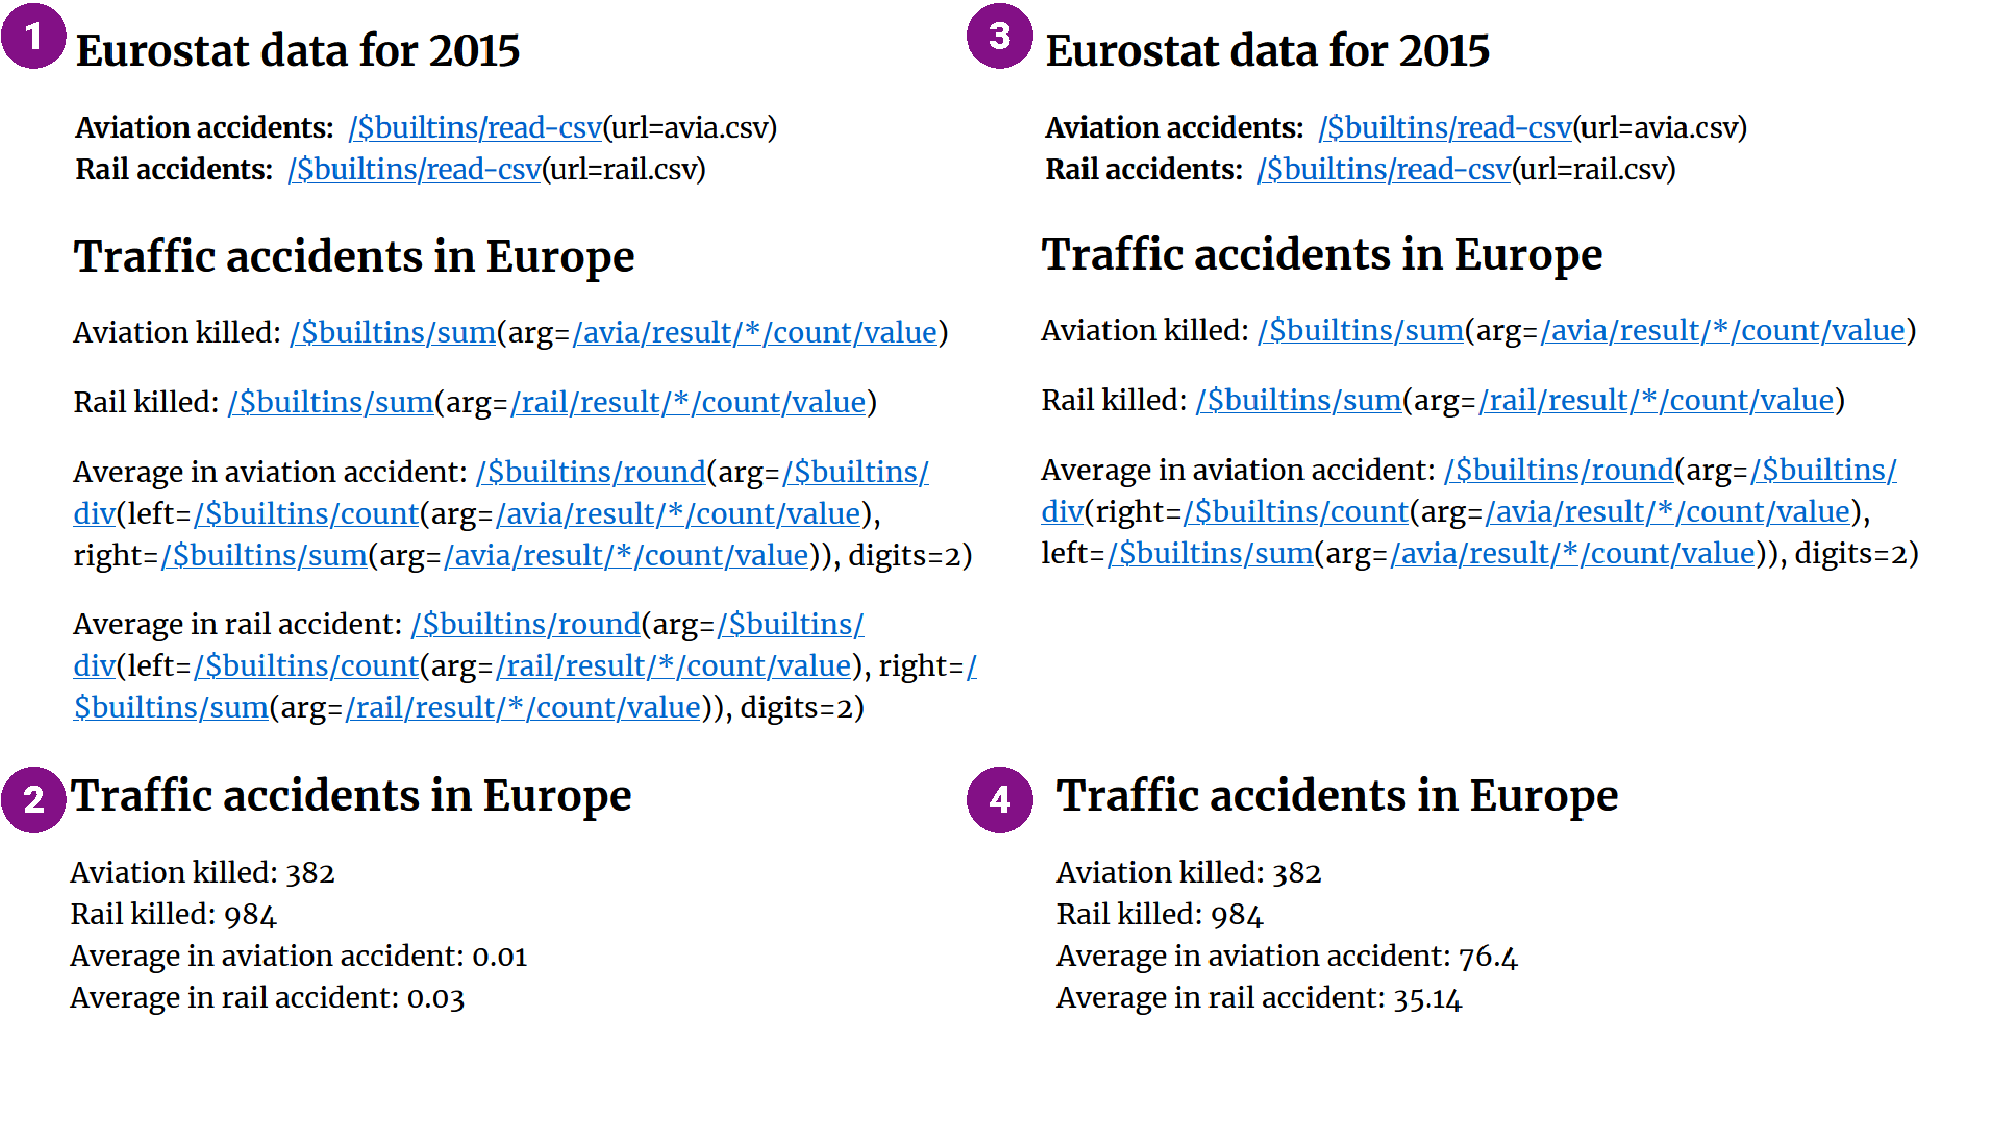
\includegraphics[width=1\columnwidth,clip,trim=0cm 1.7cm 1cm 0cm]{fig/copypaste.pdf}
\caption{The user uses creates a copy of a formula (1). They notice an error (2), go back in
history to switch the arguments (3), merge the change and re-evaluate both formulas (4).}
\label{fig:copypaste}
\end{figure}


% ==================================================================================================

\section{Design Considerations}
\label{sec:discuss}

The design of the Denicek substrate is the result of an iterative process in which we repeatedly
adapted the Denicek design and revisited the implementation of the Webnicek system until we obtained
a satisfactory solution for the six formative examples detailed in \S\ref{app:examples}. In this
section, we document the design challenges, many of which are shared with related systems
\cite{jakubovic-2022-ladder,edwards-2005-subtext,hall-2017-infra,omar-2021-livelits}.

\keyideabox{\faCubes}{Uniformity and Composability}{
Two guiding principles for the design of Denicek have been \emph{composability} and
\emph{uniformity}~\cite{jakubovic-2023-techdims}. The substrate should cover a large number of
scenarios using a small number of concepts. This is apparent in the design of the document
structure -- a node can represent data, code or rich text -- as well as in the role of
edits -- an edit can be a value change, a structure change, the result of user interaction
or the result of formula evaluation.
}

% The inconvenience associated with composability and uniformity~\cite{jakubovic-2023-techdims} is not
% a problem for Denicek. We view Denicek as an underlying structure on top of which more
% convenient end-user programming systems can be built. The uniform design offers a degree of open-endedness,
% making it possible to use the basic structures of Denicek in new ways, not anticipated in this paper.

\subsubsection*{Dynamic and Static Typing}
Denicek does not explicitly track the document structure (it is dynamically typed). For example, we
assume that lists are homogeneous, but do not enforce this property. A statically typed system could
enforce such properties and explicitly distinguish structural edits from value edits. This has a
theoretical appeal and it simplifies aspects of the implementation, e.g. by removing the need to
control reference updating, but it makes working with the system less akin to document editing.

The structural invariants are violated when constructing values gradually (e.g., when adding a new
speaker to a table), as well as during evaluation (wrapping {\small\Verb_<x-formula>_}
in {\small\Verb_<x-evaluated>_}). A system with static types could use a form of edit
transactions, where structural invariants are reestablished after a sequence of edits.

% A key design choice for a substrate like Denicek is whether to track the document structure
% explicitly or make it implicit. In Denicek, we assume that elements of a list node have the same
% structure (i.e.~records should have the same fields, so that they can be targetted using the \ident{All}
% selector), but we do not enforce this. Often, the property is temporarily violated when adding a
% list item, but then restored once the item is created.
%
% Keeping the structure (type information) explicit has theoretical appeal and it simplifies some
% aspects of the implementation. In particular, edits to document structure can be clearly separated
% from edits of document values. The same separation has disadvantages in that it complicates the
% edit language and it requires user interface that departs further from document editor.
% (In Webnicek, users can select all list items and edit them at once using the same mechanism as
% when editing individual list items. With explicit structure, changing a list structure has to be
% either a different kind of edit or possibly an edit of a virtual ``prototype'' element.)

% --------------------------------------------------------------------------------------------------

\subsubsection*{Expressive Selectors and Edits}
Our merge operation works on a pair of edit sequences, but it does not need access
to the current document state or history. This limits the expressiveness of edits. Denicek does not
support conditional edits (applied only when a specific condition holds), because merging would then
not be able to determine if two edits are conflicting. As a result, generalization of recorded
interactions (\S\ref{sec:impl-interaction}) has to be done at a meta level and generates a series
of individual edits. This design also limits the expressiveness of selectors. For example,
an edit targeting nodes with a specific tag (e.g., all {\small\Verb_<h3>_} elements) would also be
conditional.

\note{Respond to R3's question about avoiding edits depending on values and R1's concern about
usefulness for PBD tools.}
\diff{This limitation means that edits generated by generalized interactions (\S\ref{sec:impl-interaction})
can be only merged in limited ways (an item added to a list through merging after
invoking an action will not be affected by the action). We expect that the restriction on
expressiveness of selectors can be lifted for edits that do not modify the document structure,
but have not yet lifted this restriction in Denicek.}

% One specific design choice in Denicek is that the merge operation operates solely on two
% sequences of edits, but it does not need access to the current document state (or full edit
% histories). The reconciliation of edits (\S\ref{sec:system-ops}) is defined for two individual
% edits $e_1$ and $e_2$.
%
% This design limits the possible language of edits. We cannot, in general, support
% conditional edits (that are applied only when a certain condition holds for
% the current document state). This is because the merging operation would not be able to
% determine whether the edit is applied (and whether its effects should~take~place).
%
% One consequence of the design choice is that the generalization of recorded interactions (\S\ref{sec:impl-interaction}) has to
% be done on a meta-level (by specifying how to invoke edits, rather than through the edits themselves).
% Another consequence is that our langauge of selectors has to be abstract.
% We can target all list elements using the \ident{All} selector, but cannot combine this
% representation with a representation that explicitly lists indices of all items currently in the list.


% Denicek supports only a limited set of selectors. An absolute reference can select a record
% field (\ident{Field}), specific list item (\ident{Index}) or all list items (\ident{All}).
% Once can imagine a range of other useful selectors, for example to select list items with a
% given tag or select items satisfying other conditions.
%
% We could support such selectors for those edits that do not affect the document
% structure. However, supporting such conditional selectors in general is incompatible with our
% design decision that merging should not depend on document state. (If an edit wraps the body of all
% {\small\Verb_<h3>_} elements, we need to know the document state in order to determine whether
% we need to modify the selector pointing to an item at a specific index.)


\subsubsection*{List Indices and Ordering}
Denicek does not use numerical indices for lists. Indices are unique identifiers that have to
be provided explicitly. (Although Webnicek generates indices automatically when editing lists.)
The design supports a programming by demonstration scenario where the user adds a new list item
and then modifies it (e.g.,~when adding a speaker or a Todo item).

With numerical indices, the edits following \ident{Append} would not have a direct access to the
index of the added item. Computing a numerical index from the length of the list would require
a complex logic to update indices when merging edit operations that affect lists. An alternative
is to disallow modification of the newly added item, but this makes programming by demonstration
cumbersome.

% Denicek does not use implicit numerical indices for lists. When adding an item, the
% user (or the system built on top of Denicek) has to explicitly provide an index. This design
% is motivated by a typical programming by demonstration scenario where the user adds a
% new list item and then modifies it (adding a speaker or a Todo item). When using explicit indices,
% the edits following \ident{Append} can use the index to refer to and modify the newly added
% item. (To avoid overwriting existing items when replaying recorded edits, Webnicek replaces
% indices of newly added items when replaying recorded interactions in \S\ref{sec:impl-pbd}). \note{I don't think that was explained back there.}
%
% Using implicit numerical indices is possible, but it requires treating all list-related edits
% as operations that transform document selectors. This means adding multiple new rules to
% Figure~\ref{fig:updates}, which specifies how edits transform references. Merging then has to
% modify indices when edits add, remove or reorder list items. List order then, somewhat confusingly,
% becomes a part of document structure rather than a property of the list value.
%
% \note{I'm still unclear whether your list indices are ordinal numbers like in an array or are unique IDs. Your usage of implicit/explicit isn't obvious to me. The above paragraph seems to imply they are IDs. Note that automatically generating unique IDs in code execution can lead to nondeterminism. If you are using IDs, do they affect equality of lists?}
% The problem could also be avoided by not letting the user modify a list item after adding it.
% (We can require new items to be constructed outside of the list and then added through a
% single edit that combines the logic of \ident{Append} and \ident{Copy}.) This is easy to
% implement, but it requires unintuitive user interaction and it also does not address all
% use cases for modifying list item via index. \note{I'm still confused, but this sounds like it really isn't a solution afterall.}

To maintain order of list elements, Denicek uses a data structure inspired by the list MRDT
\cite{kaki-2019-mrdts} and requires specifying the index of a preceding item when appending
or inserting into a list. Denicek uses the same mechanism for record fields as the order of fields
may be visible to the user, for example in Webnicek where fields represent children of a HTML node.
Making the order of fields explicit ensures that it is maintained during merging.

% \subsubsection*{Ordering List Items and Record Fields}
% When list indices are not numerical and supplied explicitly, we need another mechanism for
% tracking order of list items. Denicek uses a data structure inspired by Mergeable Replicated
% Data Types \cite{kaki-2019-mrdts} and requires specifying the index of a preceding list item
% when appending to a list. However, Webnicek supplies the index of preceding item automatically.
% (If two edits append to the same list independently with the same preceding item, the order
% is non-deterministic.) \note{Why is this needed? I let the order of operations determine the list order. }
%
% Note that Denicek uses the same mechanism for record fields. Keeping record fields ordered is
% desirable because Denicek documents map directly to HTML documents and so the order is visible
% to a user. Moreover, different ways of merging edits can result in different order of adding fields
% to a record. Making order explicit ensures those result in equivalent documents.
%
% Denicek still makes a distinction between records and lists, even if the two are similar
% technically. The difference is conceptual. A list is expected to contain items of the
% same structure (that can be addressed using the \ident{All} selector), whereas record fields
% are expected to be of different types. If we unified lists and records, \ident{All} would have
% to be applicable to records too and inferring and checking document structure would be
% challenging.


\subsubsection*{Structure and Capabilities of Merging}
Denicek keeps a linear history and merging appends edits to the top of the history.
This model is akin to git rebase. An alternative is to maintain a graph of edits akin
to git merge. This would simplify recording of edits in programming by demonstration
(\S\ref{sec:impl-pbd}) as we would not need to update saved edits transformed
during merging. (Their hashes would remain the same.) However, supporting special
merge edits and non-linear history would make the basic substrate more complex.

Denicek also only supports the \emph{convergence} model of collaborative editing \cite{edwards-2025-schema}
where users have to merge all changes in order and cannot adopt selected edits (cherry
picking in git). The \emph{divergence} model would let users keep their own schema but
import all data edits. Supporting the model requires a \emph{retract} operation \cite{edwards-2021-typed}
that is dual to our edit reconciliation (given subsequent edits $e_1, e_2$, generate
$e_2'$ that has the same effect as $e_2$ but can occur before $e_1$).

\subsubsection*{Dependency Tracking}
Conflict detection in Denicek is used when merging edits, but also to implement
incremental recomputation (\S\ref{sec:impl-incremental}). Edits generated during formula evaluation
(\S\ref{sec:impl-eval}) may be \ident{Copy} edits (when evaluating a reference), but also
\ident{Add} edits (when setting the evaluation result to a computed value). \ident{Add} edits
need to record additional dependencies identifying the source of the operation arguments.
Alternative evaluation models avoid this need, but lead to a less uniform system design.

% Recall that the incremental recomputation (\S\ref{sec:impl-incremental}) is based on the
% conflict detection mechanism of Denicek (\S\ref{sec:system-ops}). When pushing edit $e_2$ through
% $e_1$, a conflict is detected if they affect overlapping targets or if $e_1$ modifies a
% document node that is a source of $e_2$, typically, the source of a \ident{Copy} edit.
%
% For edits generated during formula evaluation (\S\ref{sec:impl-eval}), we need to track an
% additional kind of dependency. Evaluating a formula that adds two numbers from two document
% location results in an edit that sets the result of the formula to the sum of the two numbers.
% The edit contains the resulting number, but we also need to record that the edit has the two
% source locations as dependencies. For this reason, Denicek makes it possible to annotate edits
% with additional dependencies. One alternative would be to introduce a special \ident{Evaluate}
% edit that would identify an operation to compute and a list of arguments, specified as a list
% of references. We choose the former to keep the set of edits smaller.

% --------------------------------------------------------------------------------------------------

\begin{figure*}[t]
\vspace{-0.5em}
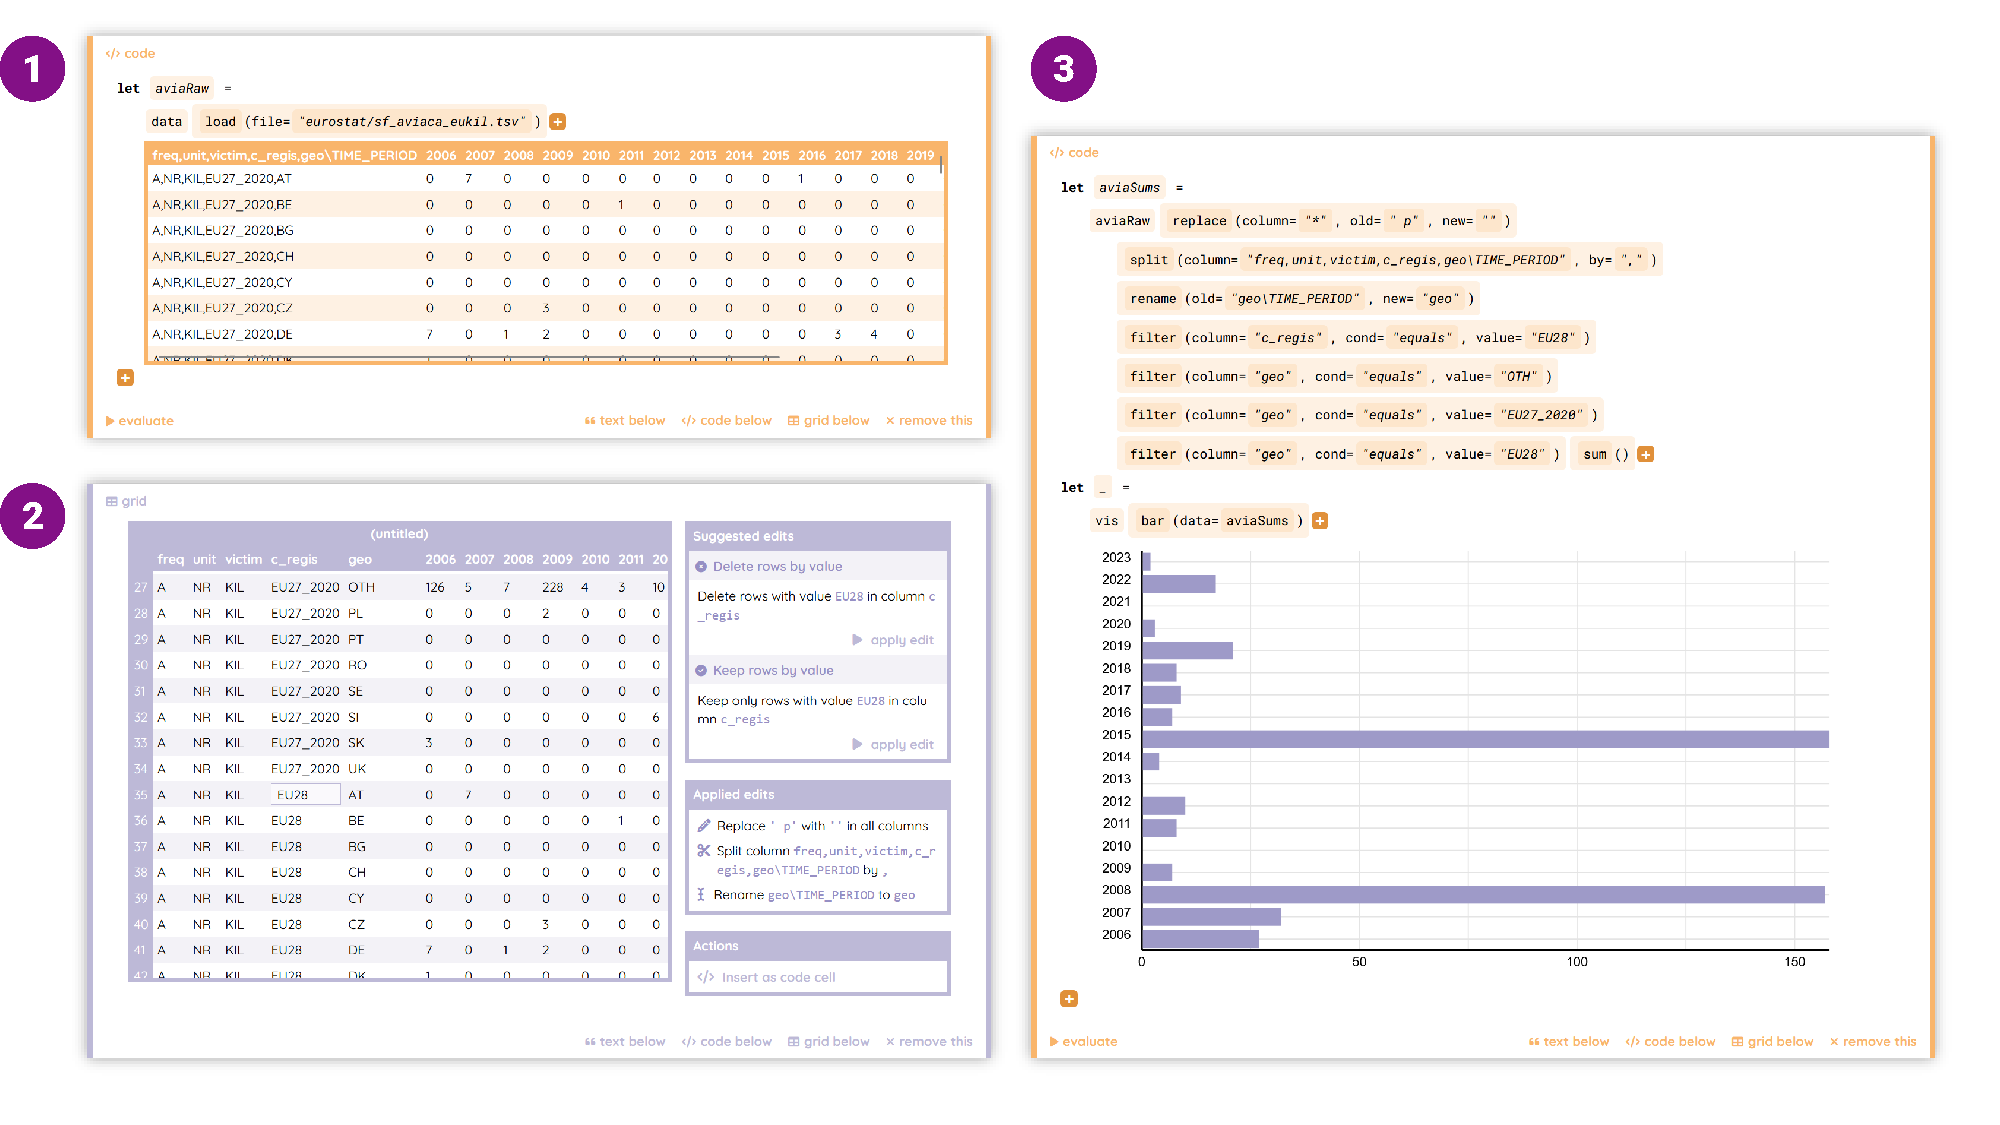
\includegraphics[width=0.98\textwidth,clip,trim=0cm 1cm 1cm 0.5cm]{fig/datnicek.pdf}
\vspace{-0.5em}
\caption{A notebook visualizing Air traffic accident data from Eurostat. The user loads data in
a code cell (1) and edits it in a grid that infers edit operations via programming by demonstration
(2). They turn the edits into a code cell (3) and add a chart.}
\label{fig:datnicek}
\end{figure*}

% ==================================================================================================

\section{Case study: Datnicek Notebooks}
\label{sec:case}

Denicek is a low-level computational substrate. It is intended as the basis for interactive
programming systems that view programs as documents. The most prominent example of such systems
today are notebook environments for data science. To explore this use case, we have developed
Datnicek, a notebook system that shows the ability of Denicek to support rich interactive user
experiences. In this section, we present Datnicek and reflect on its development. A simple data
exploration conducted in Datnicek is shown in Fig.~\ref{fig:datnicek}.

\subsection{Requirements}
\label{sec:case-req}

The design of Datnicek brings together a range of recent research ideas on interactive programming
environments for data science. Datnicek notebooks consist of code cells and markdown cells, but
they also support interactive grid cells where the user can use programming by demonstration to
construct data cleaning scripts. We aim to support the following features:

\begin{itemize}
\item \emph{Structure Editing.} Code in code cells should be edited through structure editor
  as in Histogram \cite{petricek-2019-histogram}. This allows Datnicek to keep track of the code
  structure and potentially makes the system accessible to non-programmers \cite{mcnutt-2023-projectional}.
  We do not initially aim to implement advanced keyboard-based editing \cite{moon-2022-tylr,beckman-2023-sandblocks}.

\item \emph{Collaborative Editing.} It should be possible to merge independently done code changes
  as in Grove~\cite{adams-2025-grove}, addressing the known pitfall of versioning Jupyter
  notebooks~\cite{singer-2020-jollity}.

\item \emph{Code Completion.} During editing, code completion should offer available data
  transformations and operations as when using type providers \cite{syme-2013-inforich} or
  iterative prompting in The Gamma \cite{petricek-2022-thegamma}.

\item \emph{Output Invalidation.} When code is edited, the previously evaluated results that
  depend on it, directly or transitively, should be invalidated as in Wrattler \cite{petricek-2018-wrattler,petricek-2020-live},
  addressing another well-known limitation of Jupyter notebooks \cite{koop-2017-dataflow}.

\item \emph{Interactive Data Cleaning.} It should be possible to edit tabular data in an interactive
  grid and use programming by demonstration for common cleaning tasks as in
  Wrangler or Vizier~\cite{kandel-2011-wrangler,kennedy-2022-vizier}.

\item \emph{Wrangling Code Synthesis.} Interactively constructed data transformations should be
  convertible into code that can be checked by the data scientist and further edited as in Wrex \cite{drossos-2020-wrex}.
\end{itemize}

\noindent
The Datnicek notebook system implements the above requirements on top of Denicek.
Although Datnicek is a proof of concept, it shows that Denicek provides a suitable basis
for the implementation.

% --------------------------------------------------------------------------------------------------

\subsection{Implementation}
Datnicek is implemented using the Elm architecture \cite{fowler-2020-mvu},
where a system maintains a state that is updated through events. The state consists
of the list of Denicek edits, transient state of the user interface, current computed document
and other cached information. All interactions that affect the notebook trigger
the same type of event that appends edits to the list of Denicek edits. Remaining events
update the transient user interface state. The support for collaborative editing is
implemented through an ad-hoc mechanism.

\subsubsection*{User Interface}
Datnicek notebooks consists of a series of cells. In code cells, the user can
use the ``+'' button to add a new variable, add an operation to the end of an existing chain
of operations, but also to specify an argument of an operation. The button opens
a menu showing all valid options based on the current context.

In the interactive grid, the user can edit column headers and table cells. When they edit
a value, Datnicek suggests generalised edits to be applied to the entire
column or table. For example, when the user changes the ``0 p'' value to ``0'', Datnicek
suggests to replace `` p'' with the empty string in all cells. Other suggested edits include renaming
or deleting a column, splitting a column using a delimiter and filtering rows based on the selected
value. Datnicek can also turn edits performed interactively into a new code cell.

\subsubsection*{Programmatic Code Cells}
A Denicek document representing a Datnicek notebook is shown in Fig.~\ref{fig:source}. A
notebook is a record storing individual cells as fields. The tag determines the type of the cell.

The programming language used in code cells is inspired by the data exploration calculus \cite{petricek-2020-live}.
A cell consists of a sequence of bindings of the form $\textnormal{\ident{let}}~v=e$ that assign
an expression $e$ to a variable $v$. An expression can be a reference to a variable,
global value (such as \ident{data} and \ident{vis}) or a method invocation $e.m(e_1, \ldots, e_n)$.

Bindings are represented as fields of a record and expressions use the formula representation
discussed in \S\ref{sec:impl-eval}. Operations and global values are identified by an absolute
reference pointing to the special \ident{/\$datnicek} namespace. Chains of method calls are
represented using nested formulas. Evaluation of formulas proceeds as in Webnicek
and wraps {\small\Verb_<x-formula>_} in {\small\Verb_<x-evaluated>_}.
The user interface displays the original formula alongside with the evaluated result, supporting
tables and Compost data visualizations \cite{petricek-2021-compost}. Edits to the formula
invalidate dependent results as discussed in \S\ref{sec:impl-incremental}.

\subsubsection*{Interactive Grid Cells}
Grid cells consist of a reference to the data source they edit and a collection of
{\small\Verb_<transform>_} nodes that represent individual data transformations constructed via
programming by demonstration. A transformation consists of metadata,
a sequence of edits and a formula representing the transformation (with {\small\Verb_<x-hole>_}
standing for the data table to be transformed).

A single transformation may correspond to multiple underlying Denicek edits. For example, splitting a
column named ``foo/bar'' with values of the form ``7/5'' using ``/'' as the delimiter adds a new column ``bar'', copies values from
``foo/bar'', renames ``foo/bar'' to ``foo'' and then transforms the values in the new columns
by dropping the part before and after the delimiter, respectively.

Interactive grid also supports transformations that affect rows satisfying a given
condition (e.g., deleting rows with a specific value in a given column). As discussed
in \S\ref{sec:system-defs}, Denicek does not support conditional selectors.
To implement conditional transformations, we add a special kind of (virtual) edit
{\small\Verb_<x-expandable-edit>_} that stores the underlying edit and a condition.
As in \S\ref{sec:impl-interaction}, when applying the edit, Datnicek finds all rows for which the
condition holds and generates a single non-conditional edit for each such row.


% --------------------------------------------------------------------------------------------------

\begin{figure}[t]
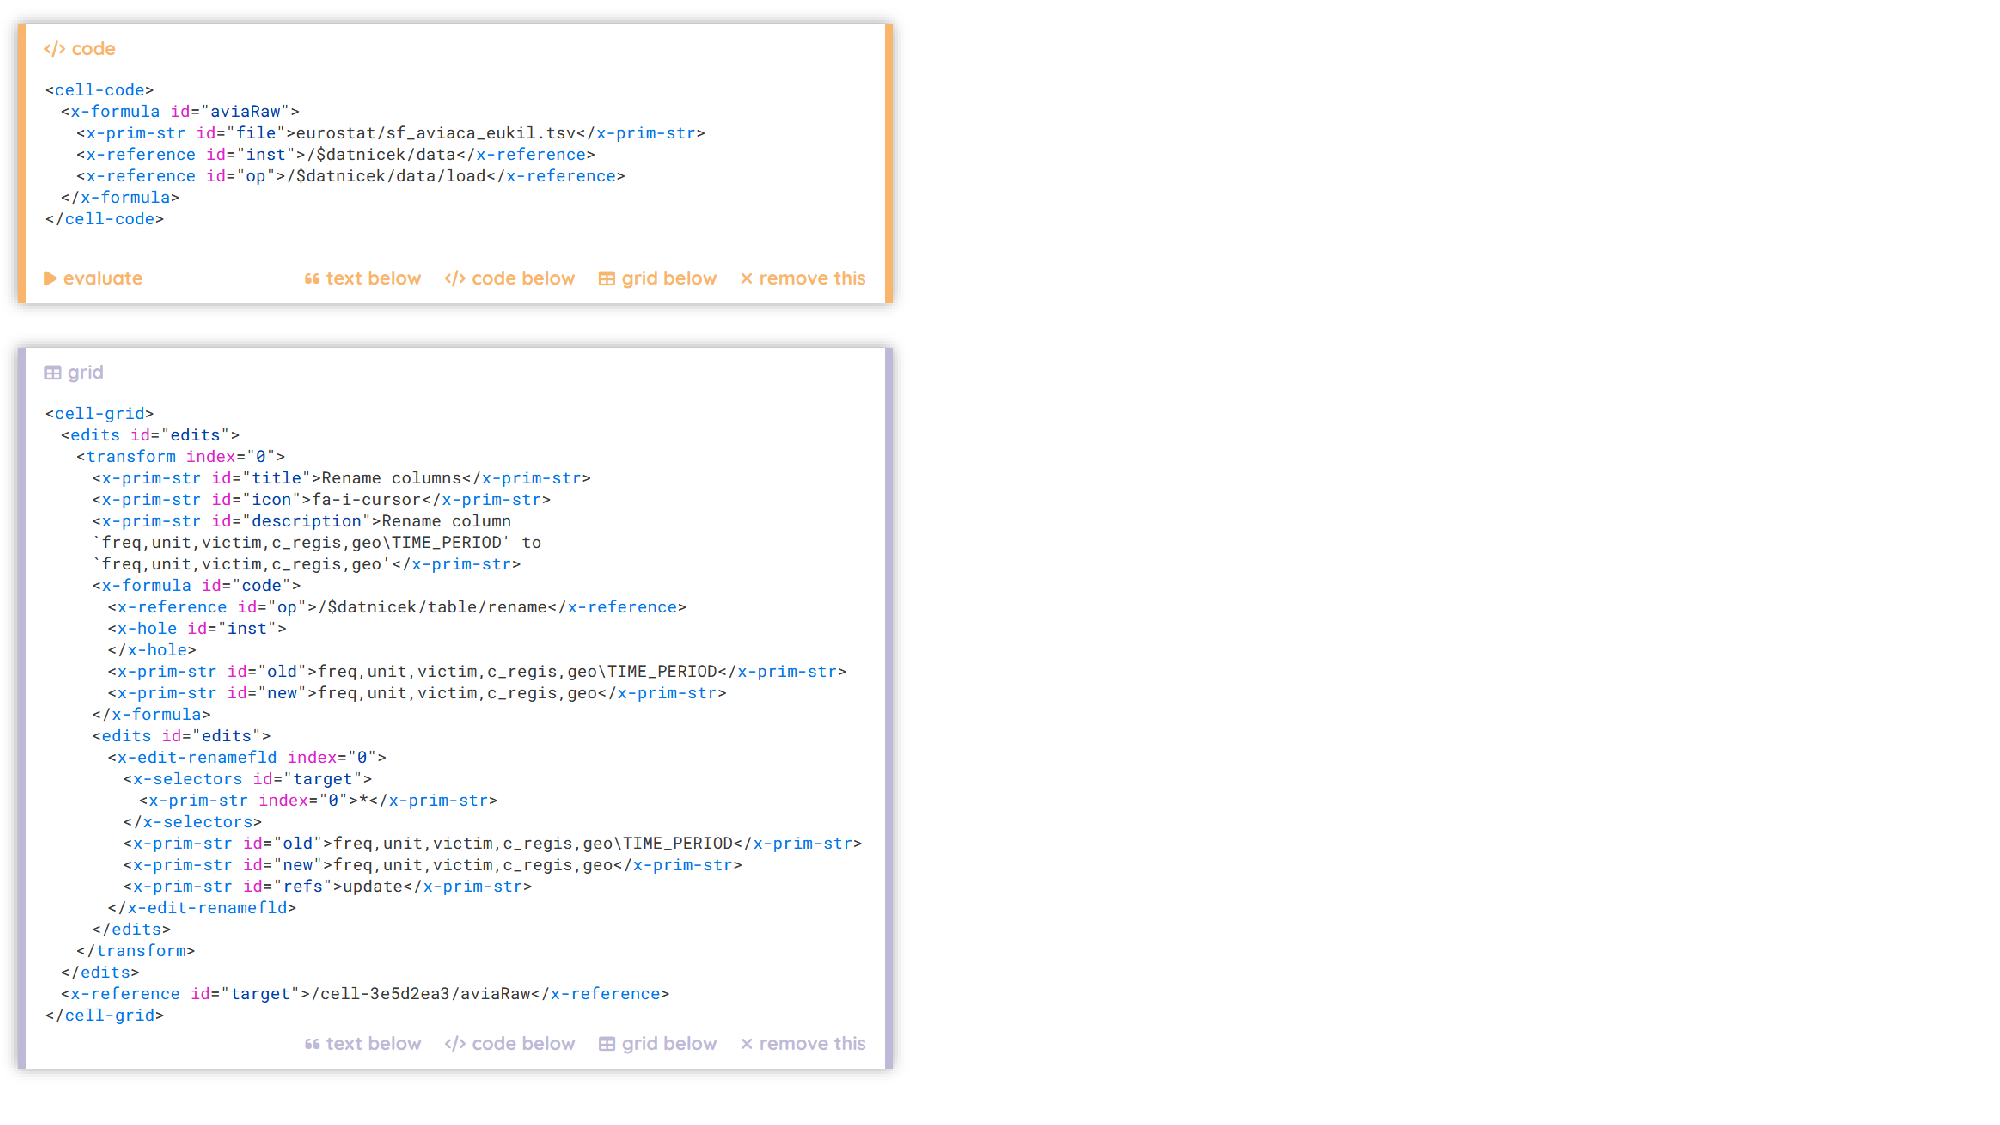
\includegraphics[width=0.9\columnwidth,clip,trim=0cm 0.7cm 18.5cm 0.2cm]{fig/source.pdf}
\caption{Underlying document representation of a code cell and a grid cell in the Datnicek
notebook system.}
\label{fig:source}
\end{figure}

% --------------------------------------------------------------------------------------------------

\subsection{Reflections}
\label{sec:case-reflection}

\subsubsection*{External Validity.}
The development of Datnicek was only started after the design and implementation of Denicek and
Webnicek was completed. Thanks to this two-phase methodology, the case study provides
a qualitative evaluation of Denicek's capabilities. \diff{The design of Denicek is based
on third-party research (\S\ref{sec:case-req}) and so the case study provides a limited external
validation. However, several design choices of Datnicek align it with the capabilities of Denicek.
This includes the use of a structure editor and
a user interface for programming by demonstration that suggests edit operations. We revisit the
generality of Denicek in \S\ref{sec:eval-tdps}, but establishing external validity ultimately
requires adoption of the open-source Denicek package by other programming system researchers.}
\note{Added discussion on external validity - although this is necessarilly limited.}

\subsubsection*{Effectiveness and Uniformity.}
Many of the Datnicek requirements are addressed by Denicek with minimal development
effort. Denicek also provides a small and uniform set of primitives. In particular,
the implementation represents all non-transient changes to a notebook as Denicek edits.
Code completions offered by the code editor are edits (wrapping a formula or appending a parameter),
changing a primitive value is an edit, and recommendations in the interactive grid are also edits
(appending a {\small\Verb_<transform>_} node).

The uniform and dynamic nature makes the development experience of using Denicek more akin to dynamic
object-oriented languages than to statically-typed functional languages. The system can quickly evolve,
but it needs suitable debugging tools, such as the source view (Fig.~\ref{fig:source}) or an
ability to step through the history.


\subsubsection*{Notebook Editing.}
Collaborative editing based on merging of edits makes conflicts less common when compared to
textual merging. For example, changing a method parameter can be merged with adding a call
to a chain. However, adding two independent calls still results in a conflict. A formula
representation that avoids nesting \cite{petricek-2019-histogram} may eliminate an even larger
proportion of conflicts.
%
Variables are represented as references and automatic reference updating %(\S\ref{sec:system-defs})
prevents a number of errors. References are automatically updated when the field (variable) name changes
and Denicek prevents the deletion of cells that contain variables to which there are references.

The proof of concept nature of Datnicek means that it currently lacks suitable user interface for
resolving conflicts. Similarly, the structure editor for code is pointer-based and would benefit from
a better support for keyboard-based input \cite{moon-2022-tylr,beckman-2023-sandblocks}.
However, Denicek provides a suitable infrastructure for implementing this.

\subsubsection*{Evaluation Model}
The evaluation model of Denicek implements dependency tracking and incremental recomputation,
which aid notebook reproducibility \cite{petricek-2018-wrattler,koop-2017-dataflow}. As in
Webnicek (\S\ref{sec:impl-incremental}), Datnicek keeps evaluated edits on top of the current history
and uses conflict detection to remove invalidated edits. We uses the same logic to evaluate
edits performed in interactive grid cells, suggesting that the approach is a useful general
implementation pattern.

However, as invalidation of evaluated edits is not built into Deni\-cek, it is worth investigating
if Denicek could support the standard evaluation model of Jupyter notebooks based on mutable state.

The development of Datnicek uncovered some limitations of conflict detection in Denicek.
In particular, edits generated by evaluation (such as \ident{Add} edits that set the
result) need to be treated as conflicting with overlapping edits with both value and structure
effects. This is because evaluated edits are the result of evaluation that considers both value
and structure of source nodes.

Finally, data loaded in Datnicek is represented as Denicek nodes (a table is a list of
records). Such uniform representation makes De\-ni\-cek more versatile, but places a high demand on the
system performance. We implemented a few basic Denicek optimisations, but Datnicek is still cumbersome
to use with data consisting of multiple thousands of rows.

\subsubsection*{Future Work}
One of the design choices discussed in \S\ref{sec:discuss} is whether to track the document
structure explicitly. The structure of documents created in Webnicek can be irregular,
which justified the dynamic nature of Denicek. In contrast, Datnicek notebooks are more regular.
Replicating Datnicek using a system akin to Denicek, but based on explicit structure would
yield an interesting comparison.

Our experience with conflict detection shows the importance of getting the details of the
implementation of programming substrates like Denicek right. This could be aided by the
development of a formally tractable model of the system and proving a correctness property
akin to that of The Gamma live previews \cite{petricek-2020-live}.

Finally, the representation of transformations in interactive grid cells (Fig.~\ref{fig:source})
highlights an unnecessary duplication -- a transformation stores a sequence of edits, as well as a formula.
Unifying these two notions is another interesting future direction.

\section{Evaluation}
\label{sec:eval}

The Datnicek case study provides a primary qualitative evaluation of Denicek. We complement this
with heuristic evaluation according to the criteria proposed by Olsen \cite{olsen-2007-evaluation}
and through the technical dimensions of programming systems framework (TDPS) developed by Jakubovic
et al. \cite{jakubovic-2023-techdims}. Criteria and dimension names are in bold.

\subsection{Complex System Evaluation}
First and foremost, Olsen \cite{olsen-2007-evaluation} argues that a system must illustrate
its \textbf{importance} for a particular class of users performing certain tasks in a given situation.
Denicek is designed to support programmers and researchers developing novel interactive programming systems,
an active research area, arguably constrained by the dependence on existing programming languages and systems.

To support a wide range of novel systems, Denicek must satisfy Olsen's criterion of \textbf{generality}.
We show that Denicek is suitable for building two very different kinds of programming systems, Webnicek
and Datnicek. We further delineate the space of supported programming systems in the next section using TDPS.

Denicek makes it easy to try different solutions, satisfying the \textbf{flexibility} condition.
This was experienced during the development of Datnicek, where a uniform representation (everything
is an edit) made it possible to quickly prototype different designs.

For an emerging class of programming systems built around documents, such as Potluck \cite{litt-2020-potluck}
and notebooks for data science, Denicek provides \textbf{expressive match} by being nearer to the
problem being solved, i.e., by using document representation for a programming system built around
documents.

Denicek also satisfies the \textbf{inductive combination}
criterion by offering a small set of primitives from which different designs can be built.
Specifically, we used Denicek to build a document-based programming system, interactive
grid for data cleaning and a structure editor with contextual code completion.

Several Olsen's criteria point to limitations of our work. First, it is unclear if Denicek
can empower new participants to be involved in programming system design. Second, the Datnicek
case study did not address scalability, although there is arguably a number of domains for which
the capabilities of the system already suffice.

\subsection{Technical Dimensions}
\label{sec:eval-tdps}

The technical dimensions (TDPS) framework \cite{jakubovic-2023-techdims} maps the design space of
interactive programming systems. We use the framework to characterize the generality of the
substrate.  For some dimensions, Denicek can cover the full range of options, while for others,
it is limited to one fixed design or a subset of options.

\subsubsection*{Interaction}
In both Datnicek and Webnicek, there is one primary \textbf{mode of interaction}. Both
systems offer immediate feedback during editing, meaning there is one main \textbf{feedback loop}.
Denicek could be used to build systems with multiple modes of interaction and feedback loops
(e.g., by separating editing, checking of edits and evaluation), but it is unsuitable for live
systems that preserve evaluation state during source code editing \cite{burckhardt-2013-live}.

Denicek covers the full range of \textbf{abstraction construction} approaches.
Abstraction \emph{from concrete cases} can be implemented via programming by demonstration as
shown in \S\ref{sec:impl-pbd} and \S\ref{sec:case}. Although Datnicek code cells do not currently
support function declarations, these could be added to provide abstraction \emph{from the
first principles}.

\subsubsection*{Notation}
Denicek supports both \textbf{notational structures}. \emph{Complementing notations} use
distinct representations for different aspects of a program. For example, Datnicek combines code cells with
interactively constructed transformations in grid cells. \emph{Overlapping notations} allow editing
of the same underlying structure in multiple ways. Although not integrated in a single system,
formula editor in Webnicek and code editor in Datnicek illustrate this option.

Even though Denicek's underlying conceptual structure is based on composability with a small number of
primitives, this does not determine \textbf{uniformity of notations} of systems built on top
of Denicek. These can support representations formed by a small set of primitives, as well as
by a large set of domain-specific constructs.

In Denicek, the \textbf{surface and internal notation} are typically closely related. The
internal notation has an explicit structure (document nodes), which can directly encode the surface
notation. Using an unstructured representation (such as text) is possible, but would be
incompatible with other Denicek capabilities such as merging.

\subsubsection*{Conceptual Structure and Customizability.}
On the scale of \textbf{conceptual integrity vs. openness}, the Denicek substrate favors integrity.
Systems based on Denicek need to use its representation of documents and document edits. This reduces
complexity, but leads to incompatibility with existing software stacks.

Systems built using Denicek currently do not exhibit the \textbf{self-sustainability} property,
i.e., the ability to be modified from within themselves. Supporting this is an appealing
possibility. A further research on the Denicek computation model should attempt to make it possible
to implement formula evaluation as, for example, conditional edits recorded in the document itself
through programming by demonstration.

% ==================================================================================================

\section{Conclusion}
Many recently developed programming experiences make the task easier, less error-prone,
more direct and more collaborative. We believe that many more research advances are possible.
Alas, novel programming experiences are difficult to implement on top of
existing programming languages. A suitable computational substrate can
significantly reduce the implementation effort needed to implement novel programming experiences.

To this end, we present Denicek, a computational substrate that represents programs as sequences
of document edits. We describe the design of Denicek and show how it supports a range of
programming experiences. A remarkable property of the design is that many programming experiences are
implemented through a straightforward combination of three basic operations provided by Denicek, namely edit
application, merging of histories and conflict~detection.

To evaluate the usability of Denicek for the development of interactive programming systems,
we use it as the basis for Datnicek, a data science notebook system that supports a range of
programming experiences pioneered in recent research systems. We also assess the substrate and
its generality through heuristic evaluation.

The design of Denicek resolves a number of challenges that have been faced by authors of related
systems, but have never been explicitly documented. While we hope researchers will adopt
Denicek as a foundation for future innovative programming systems, an equally important
contribution of our work is that it documents this existing but unwritten tacit knowledge.

% ==================================================================================================

\begin{acks}
The authors thank Clemens Nylandsted Klokmose for research guidance and
attendees of the IFIP WG 2.16 meeting in Serpiano, members of the Software Architecture Group at HPI
and attendees of LIVE 2023 for feedback on the project.
Anonymous reviewers provided invaluable actionable guidance for improving the final version
of the paper. The work has been supported by the
\grantsponsor{cuni}{Charles University}{https://d3s.mff.cuni.cz/projects/primus24/}
grant \grantnum{cuni}{PRIMUS/24/SCI/021} and by the
\grantsponsor{erccz}{Czech Ministry of Education, Youth and Sports}{https://starfos.tacr.cz/en/projekty/LL2325}
grant ERC-CZ \grantnum{erccz}{LL2325}.
\end{acks}

%\bibliographystyle{plain}
\bibliographystyle{ACM-Reference-Format}
\bibliography{paper}


\appendix

\begin{figure*}
\newcommand{\extablecol}[5]{
\small{\bfseries #1} #2\; --\; #3\\
\quad \footnotesize #4 \\[-0.2em]
\quad \footnotesize Programming experiences: \emph{#5} \\[0.6em]
}
\begin{tabular}{|l|}
\hline
\\[-1em]
\extablecol{Counter App}{\cite{kiss-2014-7guis}}
  {Counter with increment and decrement buttons.}
  {The current count is represented by a formula that is modified by the buttons.
  The user can inspect the evaluation trace to see how the count was modified.}
  {Programming by Demonstration, Incremental Recomputation, End-User Debugging}
\extablecol{Todo App}{\cite{osmani-2024-todomvc}}
  {Todo with buttons to add an item and remove all completed items.}
  {Adding an item must correctly merge with independently added functionality to
   compute which items are completed and remove them based on a formula result.}
  {Collaborative Editing, Programming by Demonstration, Incremental Recomputation, Schema Change Control}
\extablecol{Conference List}{\cite{edwards-2025-schema}}
  {Managing a list of invited conference speakers and schema change.}
  {Adding speakers to a list through an in-document user interface merges with
   refactoring that turns the list into a table and separates name from an email.}
  {Collaborative Editing, Programming by Demonstration, Schema Change Control}
\extablecol{Conference Budget}{\cite{edwards-2025-schema}}
  {Calculate budget based on a speaker list or a table.}
  {References are updated  when the list is refactored. Only affected formulas
   are recomputed and the user can view elements on which the result depends.}
  {Collaborative Editing, Incremental Recomputation, Schema Change Control, End-User Debugging}
\extablecol{Hello World}{\cite{miller-2001-simult}}
  {Normalize the capitalization of two word messages.}
  {An operation to normalize the text in a list item can be recorded and applied to
   all list items or, alternatively, applied directly to all list items.}
  {Programming by Demonstration}
\extablecol{Traffic Accidents}{\cite{edwards-2022-copypaste}}
  {Compute statistics using two data sources.}
  {Formula to compute statistics can be reused with a different data source;
   error correction is propagated automatically to the copied version of the formula.}
  {Concrete Programming, Incremental Recomputation}
\hline
\end{tabular}

\caption{Formative examples used in Denicek design}
\label{fig:examples}
\end{figure*}

\section{Formative Examples}
\label{app:examples}

The design the Denicek substrate, we identified six formative examples shown in
Fig.~\ref{fig:examples}. The examples range from established industry benchmarks
(Todo and Counter apps) to cases from literature~\cite{edwards-2022-copypaste} and
problems posed as schema change challenges \cite{edwards-2025-schema}.
The Denicek substrate then co-evolved with Webnicek, a simple web-based programming environment
built (as directly as possible) on top of the substrate and was used to solve implement the
formative examples.

Many of the formative examples include a small programming challenge, such as adding
user interface to add a new speaker, a new list item or modify the count. Our aim was for
the substrate to enable solving  those through programming by demonstration.
Programming by Demonstration is often used in data wrangling
\cite{gulwani-2012-spreadsheets,drossos-2020-wrex,gulwani-2014-flash}. Our Hello World example
is only a minimalistic illustration of such use, loosely inspired by earlier work \cite{miller-2001-simult}.

\section{Merging Edit Histories}
Recall that merging takes two edit histories, $E, E_1$ and $E, E_2$,
transforms edits $E_2$ into $E_2'$ that can be reapplied on top of the first history
resulting in $E, E_1, E_2'$. The key operation takes two individual edits, $e_1$ and $e_2$
and produces a sequence of edits $e_2', e_2'', \ldots$ that can be applied after $e_1$,
and combine the two edits. This section provides details about the two aspects of this operation.

\subsection{Apply to Newly Added}
\label{app:merge-apply-to-added}

Assume that edits $e_1$ and $e_2$ occurred independently. We want to modify $e_2$ so that
it can be placed after $e_1$. If the edit $e_2$ added new nodes to the document that the
edit $e_1$ would affect, we generate an additional edit that apply the transformation of $e_1$
to the newly added nodes (and only to those).

The only edits that add new document nodes are \ident{Add}, \ident{Append}, \ident{Copy} and
so we consider this case if the edit $e_2$ is one of those. If so, we check
whether the target of $e_1$ is within the target of $e_2$, i.e., the list of selectors that
forms the target of $e_2$ is a prefix of the list of selectors that forms the target of $e_1$.

Along the way, we compute a \emph{more specific prefix}. If the target of $e_1$ contains
the \ident{All} selector, it can be matched against a specific \ident{Index} selector in the
target of $e_2$ (if the selector of $e_1$ is more specific than that of $e_2$, the targets
are not matched). We then replace the original prefix in $e_1$ with the \emph{more specific prefix}
that contains \ident{Index} selector in places where the original edit contained \ident{All}.
This way, we obtain $e_1'$ which is a focused version of $e_1$ that applies only to the
nodes newly added by $e_2$. The edit $e_2$ thus becomes a pair of edits $e_2, e_1'$.
The final document will contain edits $e_1, e_2, e_1'$ -- that is, it will first apply the edit
$e_1$ to nodes already in the document, then add new nodes and then apply the transformation
represented by $e_1$ to the newly added nodes.

\subsection{Transform Matching References}
\label{app:merge-transform-refs}

As above, assume that edits $e_1$ and $e_2$ occurred independently. We want to
modify $e_2$ so that it can be placed after $e_1$. If $e_1$ is any of the three edits
listed in Fig.~\ref{fig:updates} (\ident{RenameField}, \ident{WrapRecord}, \ident{WrapList}),
we collect all references that appear inside $e_2$ (the target, the source of \ident{Copy}
and any references occurring in the nodes added by \ident{Add} or \ident{Append}).
If the target of $e_1$ is a prefix of any of those references, we update the references
accordingly and obtain a new edit $e_2'$. Note that it would be an error to match specific
\ident{Index} in $e_1$ with more general \ident{All} in $e_2$, but this cannot happen --
reference updating is not done when the target of $e_1$ contains \ident{Index}.

Now consider the case when $e_1$ is \ident{Copy} and the edit $e_2$ targets a node that is
the source node of the copy operation (or any of its children). In this case, it is reasonable
to require that the edit $e_2$ is applied to both the source and the target of the copy.
(This is required by the refactoring done in the Conference Budget example.)
We handle the case by creating a copy of $e_2$ with transformed selectors (target and, if $e_2$
is also \ident{Copy}, also its source). To transform the selectors, we replace the prefix
formed by the source of the \ident{Copy} by a new prefix, formed by the target target of
the \ident{Copy}. We then add the new operation as $e_2'$ if at least one of its selectors
was transformed (typically target, but possibly also source).


\end{document}
